\subsection{Second-Order, Geometric, and Orthogonality Optimizers}
\paragraph{Shampoo (Matrix Preconditioning via Kronecker Products).}
\begin{figure}[H]
\centering
\fitfigure{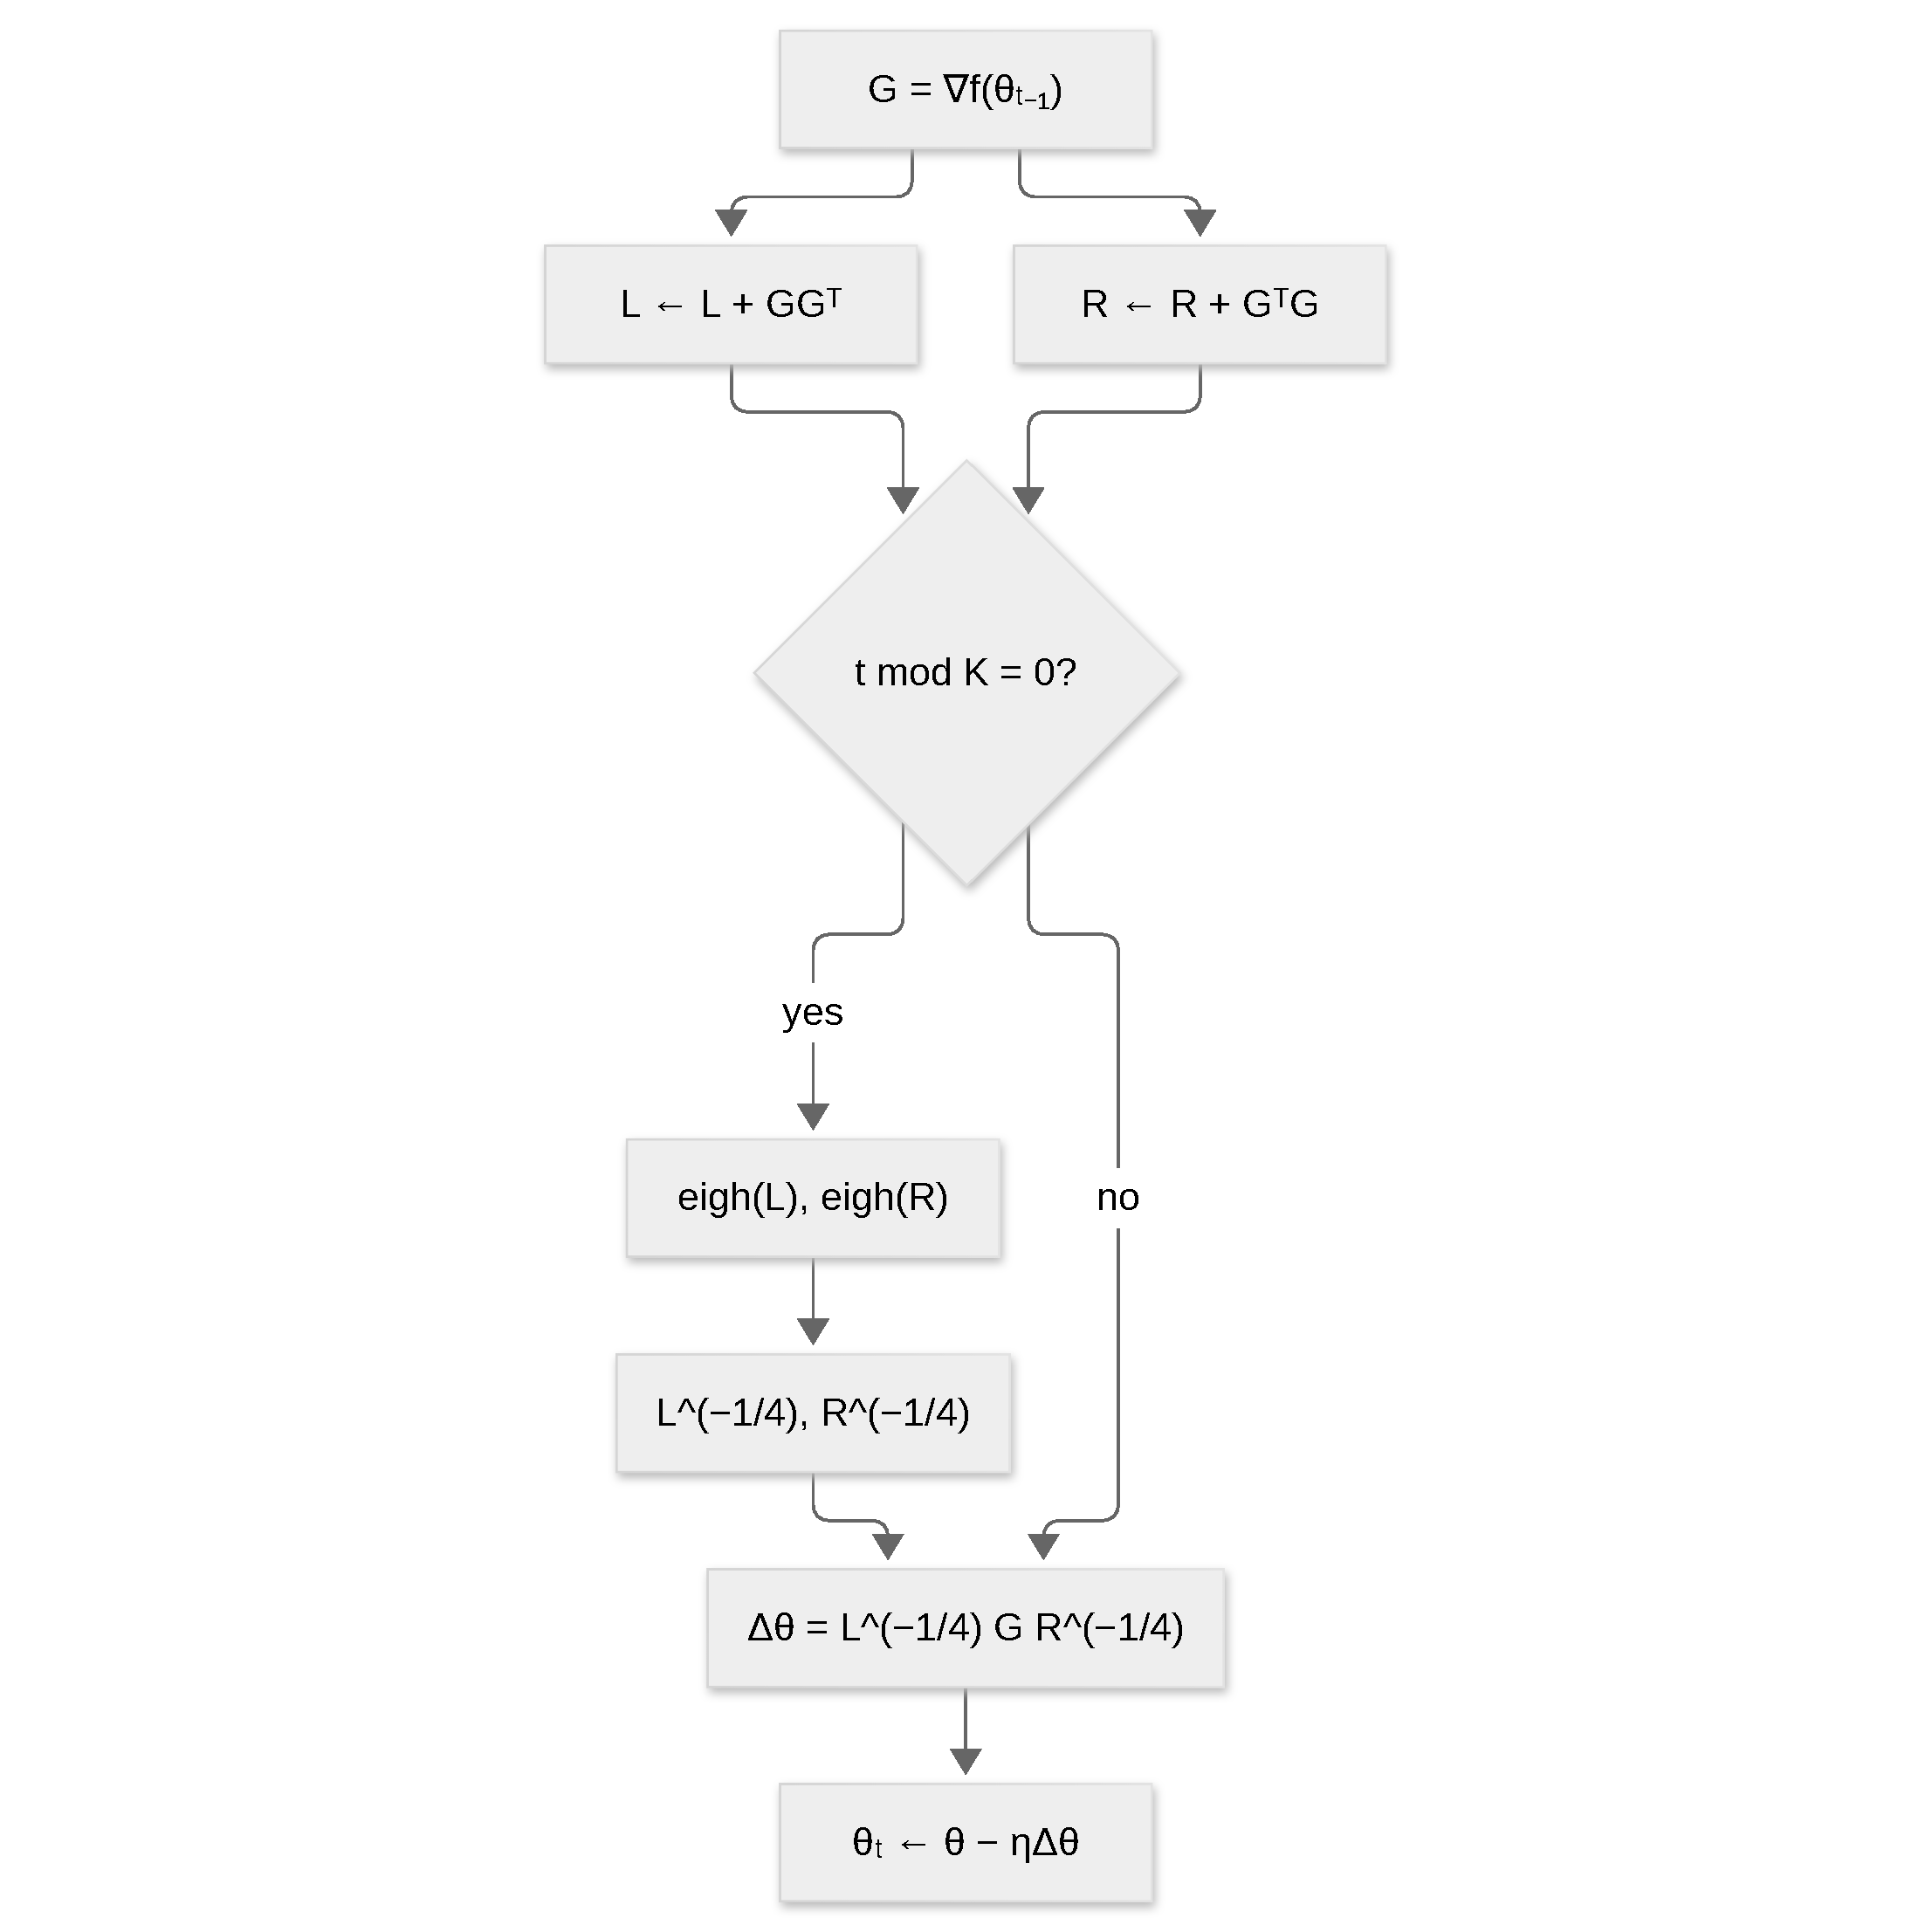
\includegraphics{figures/optimizers/shampoo.pdf}}
\caption{Step flow of Shampoo: Kronecker-factored Gram matrices, periodic eigendecomposition, and fourth-root preconditioning of the gradient.}
\label{fig:opt-shampoo}
\end{figure}
Shampoo is a \textbf{structured second-order method} that computes matrix preconditioners from Kronecker-structured outer-product statistics. For a 2D parameter matrix $W \in \mathbb{R}^{m \times n}$:
\begin{align}
L_t &= L_{t-1} + G_t G_t^\top \quad\text{(left/row Gram matrix, $m \times m$)} \\
R_t &= R_{t-1} + G_t^\top G_t \quad\text{(right/column Gram matrix, $n \times n$)} \\
L_t^{-1/4} &= Q_L (\Lambda_L)^{-1/4} Q_L^\top \quad\text{(via eigendecomposition)} \\
R_t^{-1/4} &= Q_R (\Lambda_R)^{-1/4} Q_R^\top \\
\Delta W_t &= L_t^{-1/4} G_t R_t^{-1/4} \quad\text{(preconditioned gradient)}
\end{align}
Shampoo approximates the full-matrix Adagrad preconditioner $H^{-1/2}$ (where $H$ is the Hessian) using Kronecker-factored structure. Instead of storing a $(mn) \times (mn)$ preconditioner, Shampoo maintains two smaller matrices ($m \times m$ and $n \times n$), capturing cross-parameter correlations within and across groups. Eigendecompositions are performed periodically (e.g., every $K=10$ steps) to amortize cost.

\begin{algorithm}[H]
\caption{Shampoo (Matrix Preconditioning via Kronecker Products)}
\label{alg:shampoo}
\begin{algorithmic}[1]
\Require Initial parameters $\theta_0$, learning rate $\eta$, eigendecomposition interval $K$
\Ensure Updated parameters $\theta_T$
\State Initialize: $L \gets \epsilon I_m$, $R \gets \epsilon I_n$ (left and right Gram matrices)
\For{$t = 1, 2, \ldots, T$}
    \State $G \gets \nabla f(\theta_{t-1})$ \Comment{Gradient}
    \State Update Gram matrices: $L \gets L + G G^\top$, $R \gets R + G^\top G$
    \If{$t \mod K == 0$}
        \State $Q_L, \Lambda_L \gets \text{eigh}(L)$ \Comment{Eigendecomposition of $L$}
        \State $Q_R, \Lambda_R \gets \text{eigh}(R)$ \Comment{Eigendecomposition of $R$}
        \State $L^{-1/4} \gets Q_L (\Lambda_L + \epsilon)^{-1/4} Q_L^\top$
        \State $R^{-1/4} \gets Q_R (\Lambda_R + \epsilon)^{-1/4} Q_R^\top$
    \EndIf
    \State $\Delta \theta \gets L^{-1/4} G R^{-1/4}$ \Comment{Preconditioned gradient}
    \State $\theta_t \gets \theta_{t-1} - \eta \cdot \Delta \theta$
\EndFor
\Return $\theta_T$
\end{algorithmic}
\end{algorithm}

\paragraph{Cons.}
\begin{itemize}[leftmargin=*]
\item Periodic $O(m^3 + n^3)$ eigendecompositions and higher per-step compute.
\item Assumes 2D parameter structure; embeddings and biases need separate handling.
\end{itemize}

\paragraph{Pros.}
\begin{itemize}[leftmargin=*]
\item Kronecker-factored second-order preconditioning without a dense $(mn) \times (mn)$ matrix.
\item Proven effective at production scale and well suited to high-rank transformer matrices, with improved conditioning and accelerated convergence.
\end{itemize}

\paragraph{SOAP (Shampoo with Adam in eigenbasis).}
\begin{figure}[H]
\centering
\fitfigure{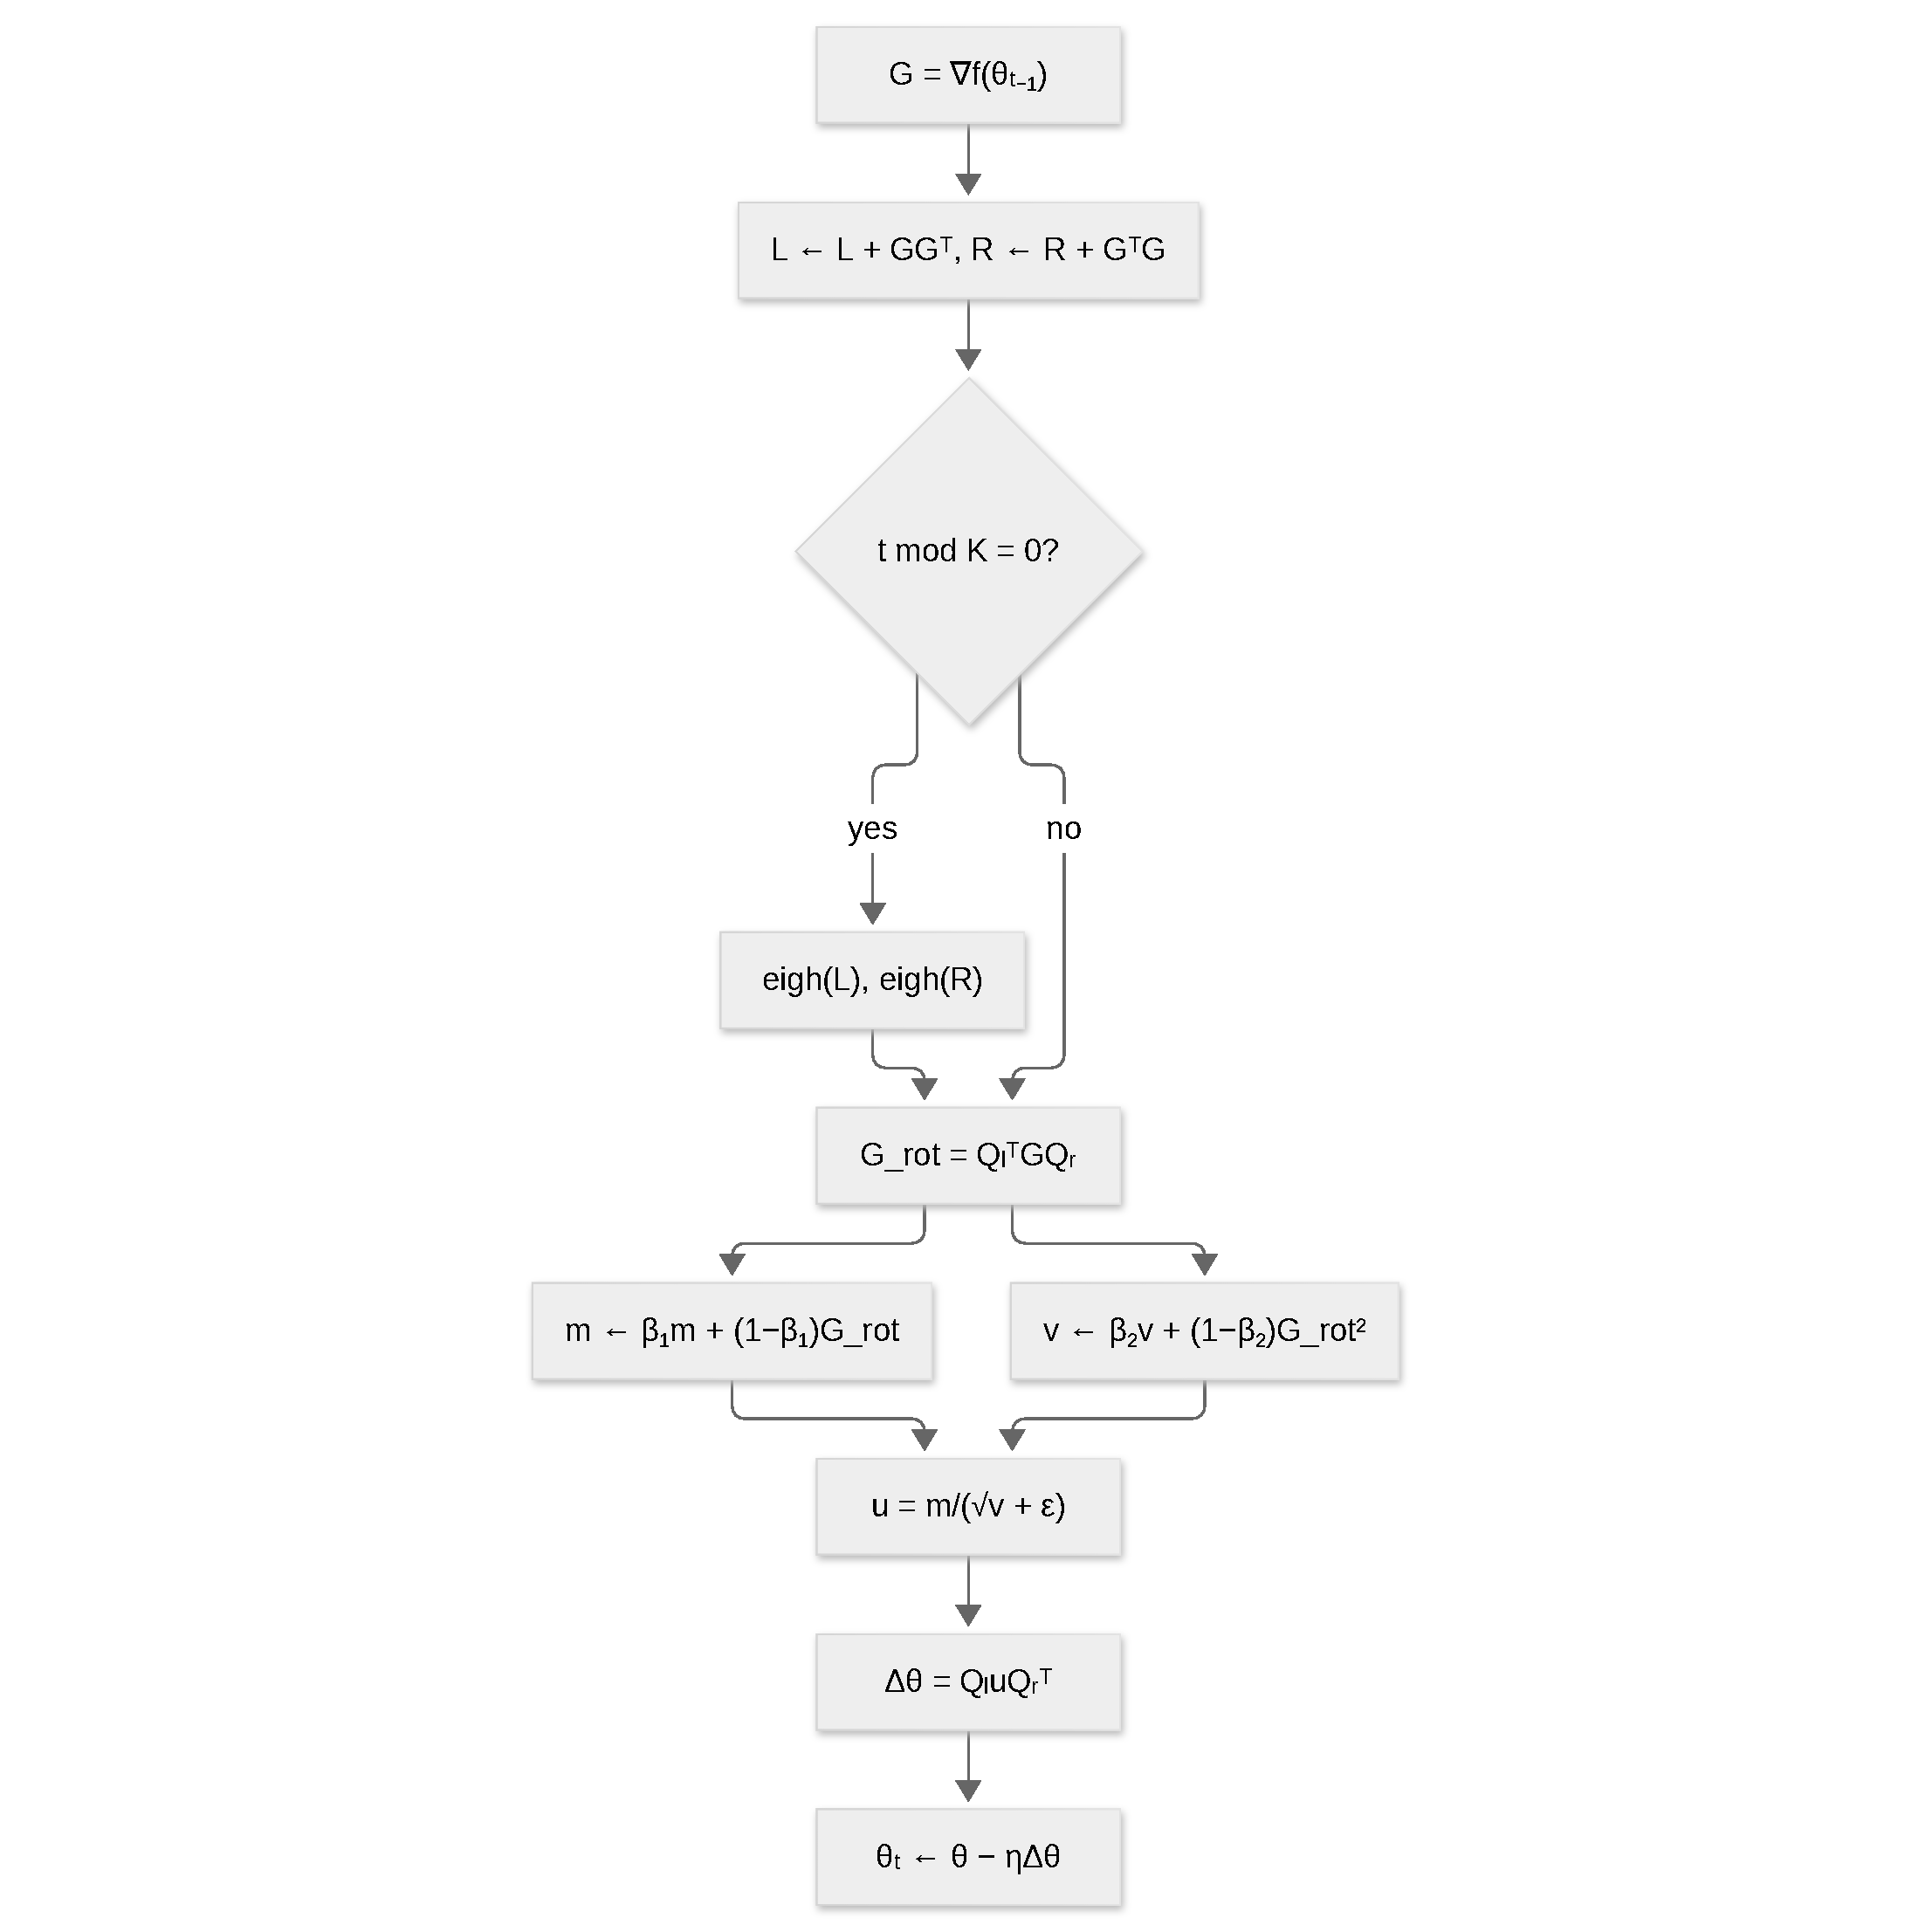
\includegraphics{figures/optimizers/soap.pdf}}
\caption{Step flow of SOAP: Adam moments tracked in the Shampoo eigenbasis and rotated back to parameter space.}
\label{fig:opt-soap}
\end{figure}
SOAP is a simplified variant of Shampoo that decouples preconditioning from momentum tracking. Instead of complex matrix algebra on preconditioned gradients, SOAP runs standard Adam in the eigenbasis of Shampoo's preconditioners:
\begin{align}
L_t &= L_{t-1} + G_t G_t^\top, \quad R_t = R_{t-1} + G_t^\top G_t \quad\text{(Gram accumulation)} \\
Q_L, \Lambda_L &= \text{eigh}(L_t), \quad Q_R, \Lambda_R = \text{eigh}(R_t) \quad\text{(periodic eigendecomposition)} \\
G_t^{\text{rot}} &= Q_L^\top G_t Q_R \quad\text{(rotate gradient into eigenbasis)} \\
m_t^{\text{rot}} &= \beta_1 m_{t-1}^{\text{rot}} + (1-\beta_1) G_t^{\text{rot}} \\
v_t^{\text{rot}} &= \beta_2 v_{t-1}^{\text{rot}} + (1-\beta_2)(G_t^{\text{rot}})^2 \quad\text{(Adam in rotated space)} \\
U_t^{\text{rot}} &= \frac{m_t^{\text{rot}}}{\sqrt{v_t^{\text{rot}}}+\epsilon}, \quad U_t = Q_L U_t^{\text{rot}} Q_R^\top \quad\text{(rotate back)}
\end{align}
The key insight: all momentum tracking occurs in the well-conditioned eigenbasis, simplifying numerical stability and theoretical analysis.

\begin{algorithm}[H]
\caption{SOAP (Shampoo with Adam in Eigenbasis)}
\label{alg:soap}
\begin{algorithmic}[1]
\Require Initial parameters $\theta_0$, learning rate $\eta$, $\beta_1, \beta_2$, eigendecomposition interval $K$
\Ensure Updated parameters $\theta_T$
\State Initialize: $L \gets \epsilon I_m$, $R \gets \epsilon I_n$, $m \gets 0$, $v \gets 0$
\For{$t = 1, 2, \ldots, T$}
    \State $G \gets \nabla f(\theta_{t-1})$ \Comment{Gradient}
    \State Update Gram: $L \gets L + G G^\top$, $R \gets R + G^\top G$
    \If{$t \mod K == 0$}
        \State $Q_L, \Lambda_L \gets \text{eigh}(L)$, $Q_R, \Lambda_R \gets \text{eigh}(R)$
    \EndIf
    \State $G^{\text{rot}} \gets Q_L^\top G Q_R$ \Comment{Rotate gradient into eigenbasis}
    \State $m \gets \beta_1 m + (1-\beta_1) G^{\text{rot}}$ \Comment{Exponential moving average (bias-correct outside)}
    \State $v \gets \beta_2 v + (1-\beta_2) (G^{\text{rot}})^2$ \Comment{Second moment (bias-correct outside)}
    \State $u \gets m / (\sqrt{v} + \epsilon)$ \Comment{Adaptive step in eigenbasis}
    \State $\Delta \theta \gets Q_L u Q_R^\top$ \Comment{Rotate back to parameter space}
    \State $\theta_t \gets \theta_{t-1} - \eta \cdot \Delta \theta$
\EndFor
\Return $\theta_T$
\end{algorithmic}
\end{algorithm}

\paragraph{Cons.}
\begin{itemize}[leftmargin=*]
\item Inherits Shampoo's periodic eigendecomposition cost.
\item Rotation and inverse rotation add matrix multiplications per step.
\end{itemize}

\paragraph{Pros.}
\begin{itemize}[leftmargin=*]
\item Combines Shampoo's explicit curvature structure with Adam's proven momentum mechanics.
\item Often cleaner and more stable than full Shampoo, with eigendecompositions amortized every $K$ steps.
\end{itemize}

\paragraph{Lion (EvoLved Sign Momentum).}
\begin{figure}[H]
\centering
\fitfigure{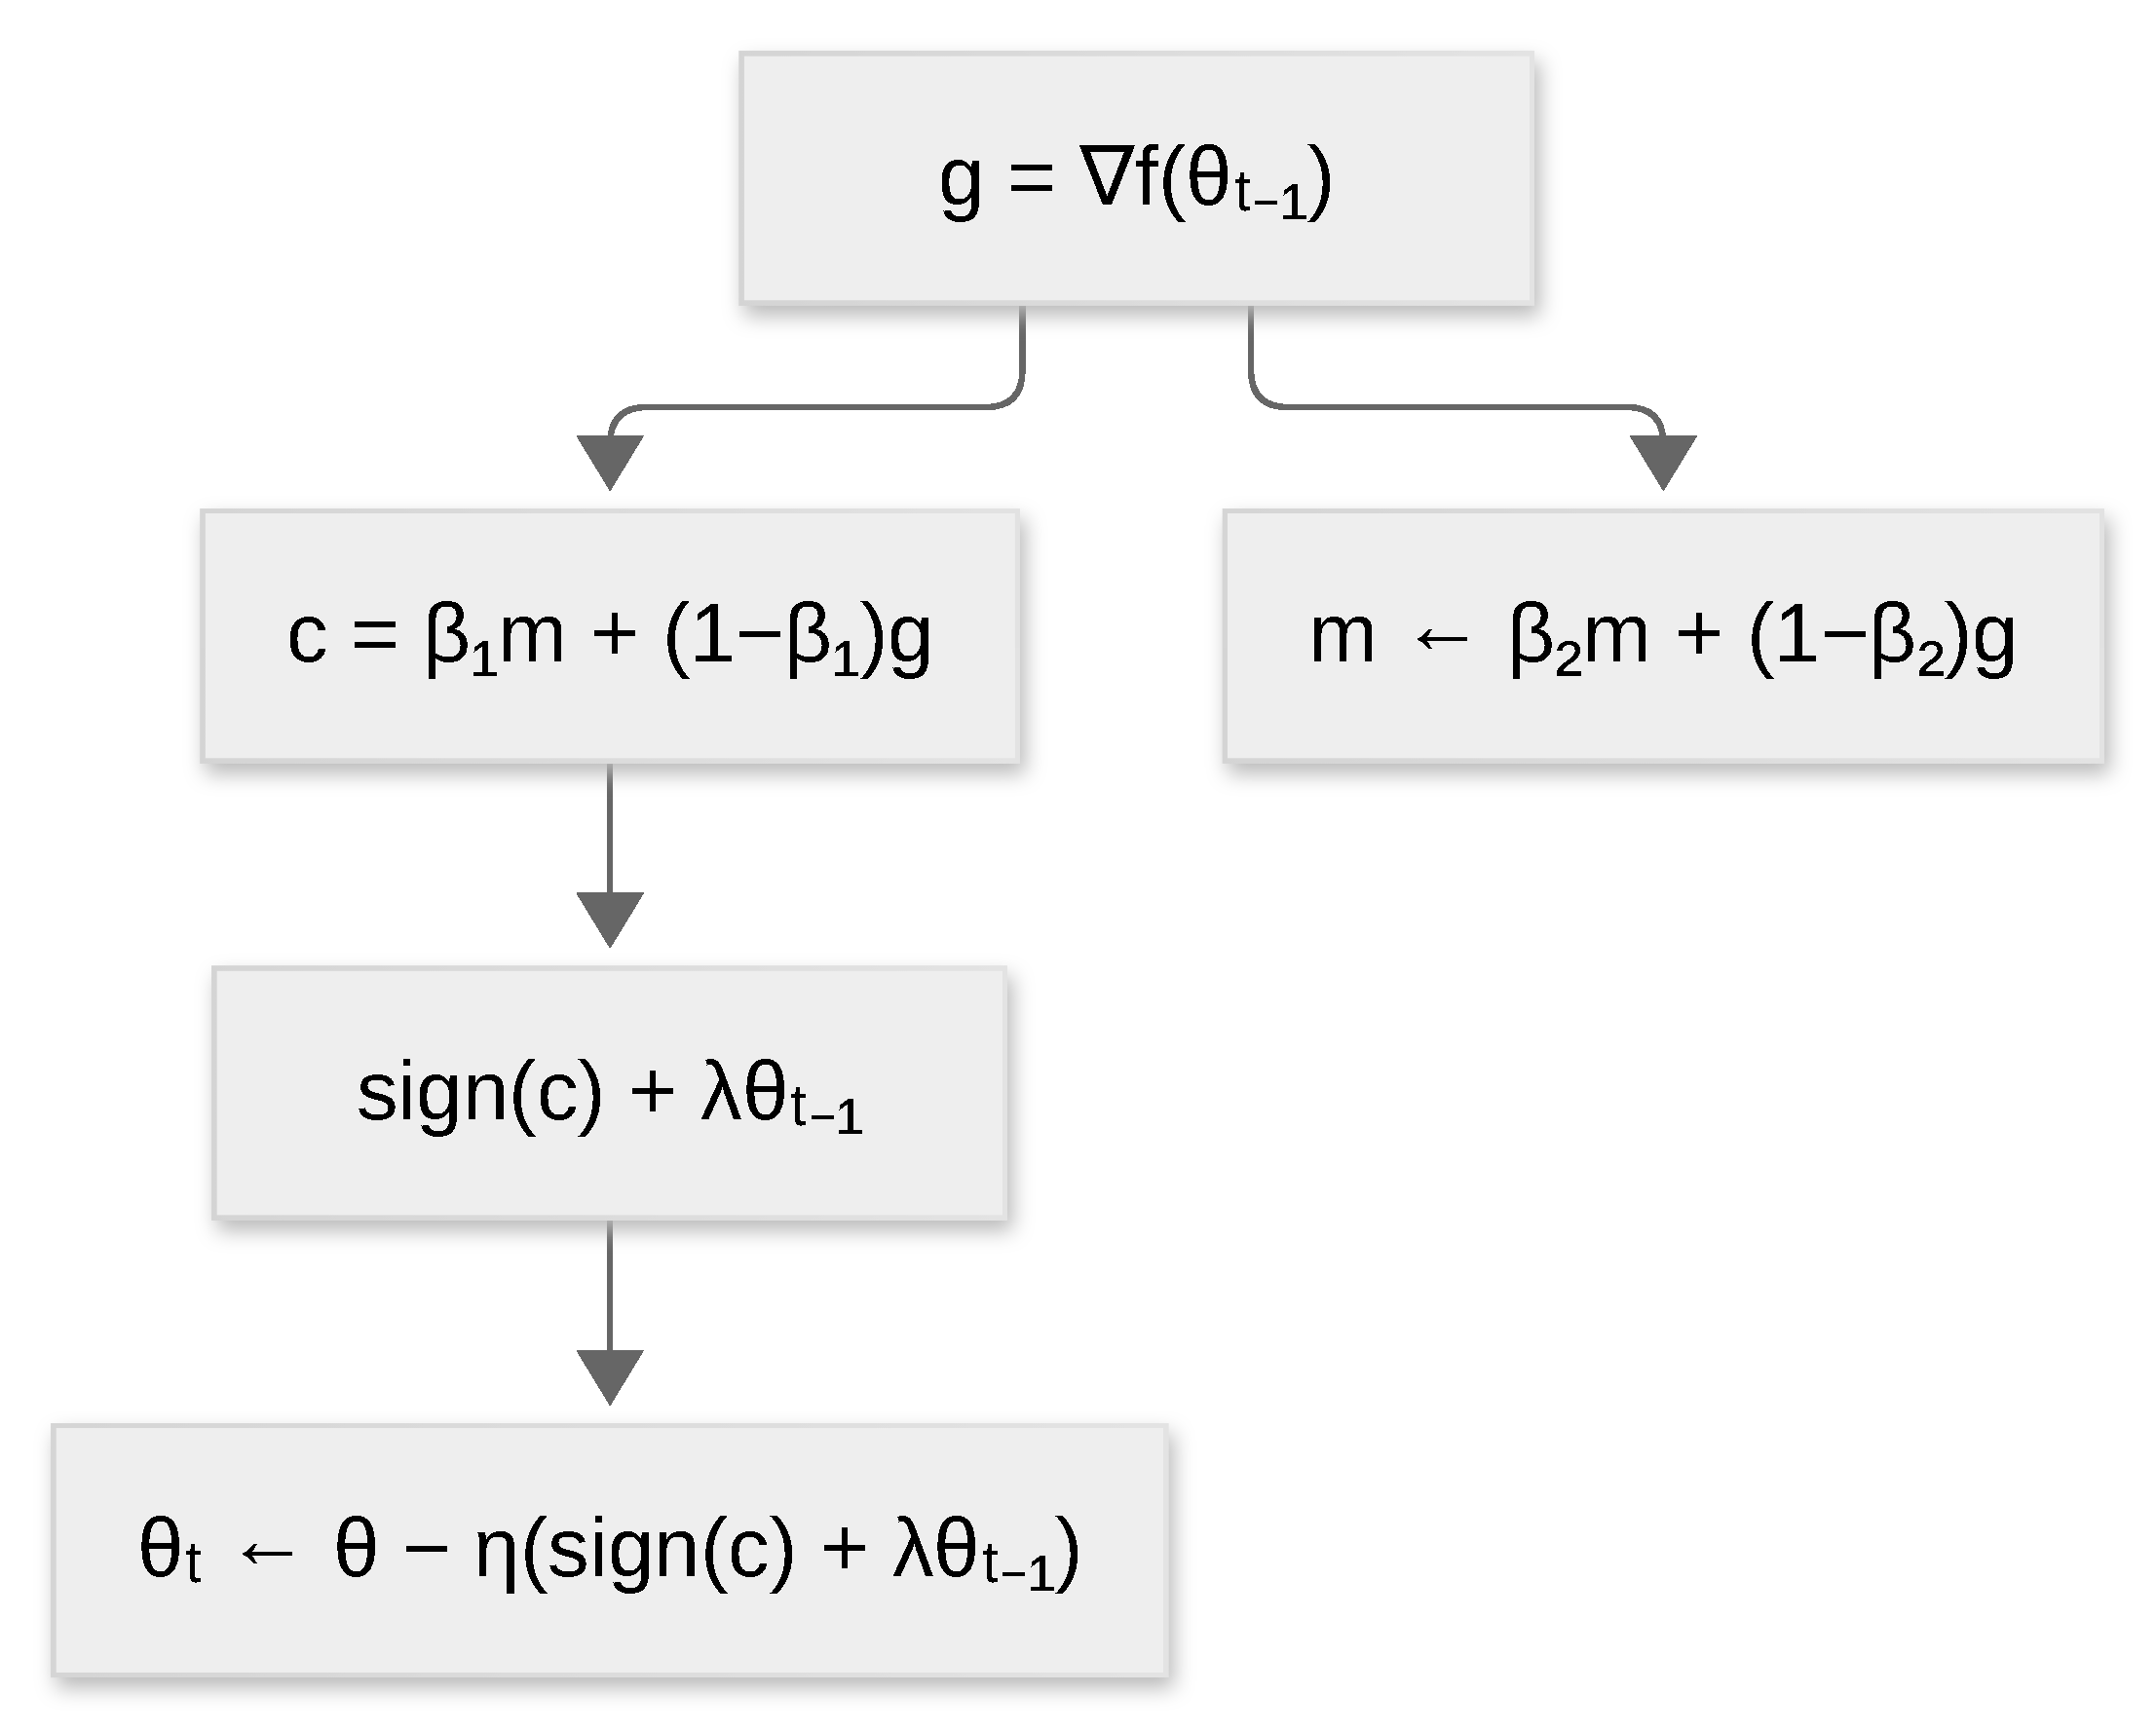
\includegraphics{figures/optimizers/lion.pdf}}
\caption{Step flow of Lion: sign-of-momentum update with decoupled momentum accumulation and weight decay.}
\label{fig:opt-lion}
\end{figure}
Lion achieves \textbf{minimal memory overhead} by using sign-based updates instead of full adaptive scaling:
\begin{align}
c_t &= \beta_1 m_t + (1-\beta_1) g_t \quad\text{(momentum input)} \\
\theta_{t+1} &= \theta_t - \eta \left(\text{sign}(c_t) + \lambda\theta_t\right) \quad\text{(sign operator update)} \\
m_{t+1} &= \beta_2 m_t + (1-\beta_2) g_t \quad\text{(momentum accumulation)}
\end{align}
All element-wise scaling operations are replaced with \texttt{sign()}, which outputs $\{-1, 0, +1\}$. This dramatically reduces memory compared to Adam-like methods: Lion stores only the momentum buffer, no second moment variance.

\begin{algorithm}[H]
\caption{Lion (EvoLved Sign Momentum)}
\label{alg:lion}
\begin{algorithmic}[1]
\Require Initial parameters $\theta_0$, learning rate $\eta$, $\beta_1, \beta_2$, weight decay $\lambda$
\Ensure Updated parameters $\theta_T$
\State Initialize: $m \gets 0$ (momentum buffer)
\For{$t = 1, 2, \ldots, T$}
    \State $g \gets \nabla f(\theta_{t-1})$ \Comment{Gradient}
    \State $c \gets \beta_1 m + (1-\beta_1) g$ \Comment{Momentum input}
    \State $\theta_t \gets \theta_{t-1} - \eta (\text{sign}(c) + \lambda \theta_{t-1})$ \Comment{Sign-based update with weight decay}
    \State $m \gets \beta_2 m + (1-\beta_2) g$ \Comment{Momentum accumulation (decoupled)}
\EndFor
\Return $\theta_T$
\end{algorithmic}
\end{algorithm}

\paragraph{Cons.}
\begin{itemize}[leftmargin=*]
\item Sign-based updates sacrifice the element-wise learning-rate adaptation that makes Adam effective.
\item Can be less robust than Adam-family methods on tasks that need adaptive scaling.
\end{itemize}

\paragraph{Pros.}
\begin{itemize}[leftmargin=*]
\item Stores only the momentum buffer, with no second moment variance.
\item High-throughput, low-memory option for large-batch regimes where activation memory dominates.
\end{itemize}

\paragraph{Sophia (Second-Order Hessian Information with Optimized Approximation).}
\begin{figure}[H]
\centering
\fitfigure{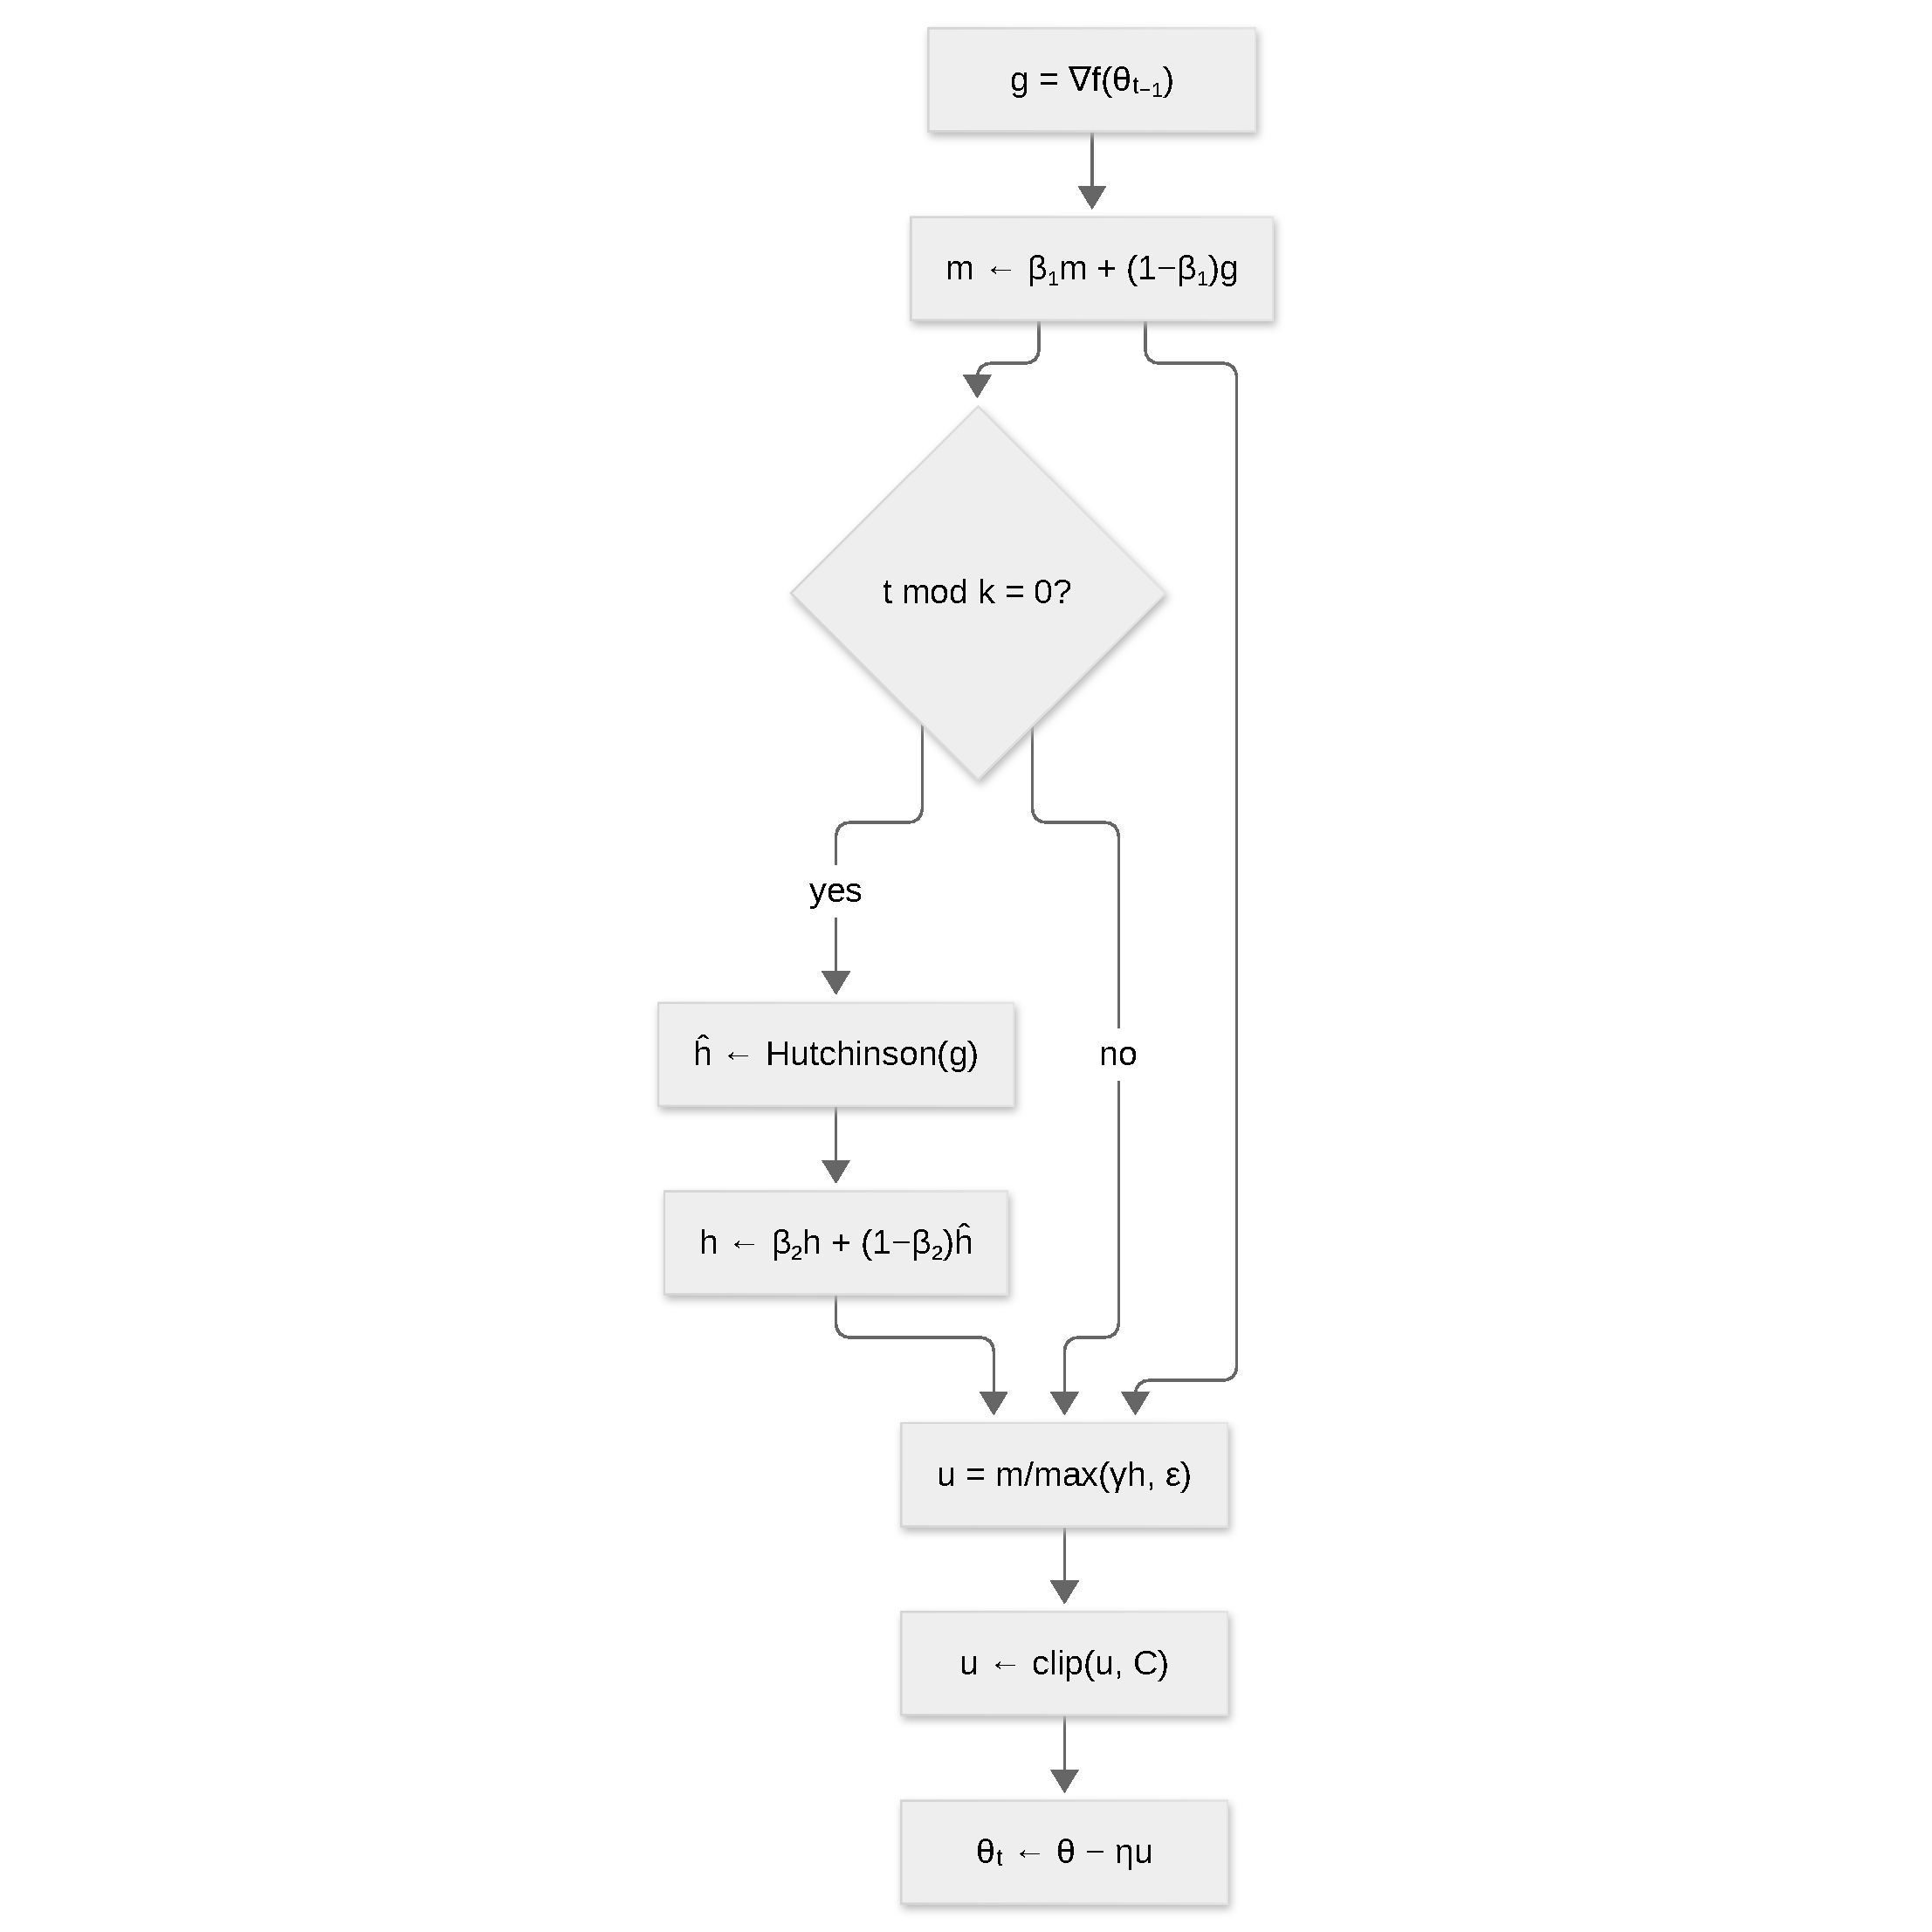
\includegraphics{figures/optimizers/sophia.pdf}}
\caption{Step flow of Sophia: diagonal Hutchinson Hessian estimate with clipped, curvature-aware element-wise steps.}
\label{fig:opt-sophia}
\end{figure}
Sophia uses \textbf{diagonal Hessian estimates} for curvature-aware scaling without the memory and compute cost of dense second-order methods.
\begin{align}
m_t &= \beta_1 m_{t-1} + (1-\beta_1) g_t \quad\text{(first moment)} \\
h_t &= \beta_2 h_{t-(k-1)} + (1-\beta_2) \hat{h}_t \quad\text{(diagonal Hessian, updated every $k$ steps)} \\
\text{clip}(x, C) &= \min(\max(x, -C), C) \quad\text{(element-wise clipping)} \\
\theta_{t+1} &= \theta_t - \eta \cdot \text{clip}\left(\frac{m_t}{\max(\gamma h_t, \epsilon)}, 1\right)
\end{align}
where $\hat{h}_t$ is a diagonal estimate (e.g., Hutchinson-trace estimator) and $\gamma$ is a scaling factor. The diagonal Hessian $h_t$ captures local curvature, allowing the optimizer to take smaller steps in sharp directions and larger steps in flat directions. The clipping operation $\text{clip}(\cdot, 1)$ prevents adaptive steps from exploding.

\begin{algorithm}[H]
\caption{Sophia (Diagonal Hessian with Clipped Updates)}
\label{alg:sophia}
\begin{algorithmic}[1]
\Require Initial parameters $\theta_0$, learning rate $\eta$, $\beta_1, \beta_2$, Hessian update freq $k$, clip threshold $C$
\Ensure Updated parameters $\theta_T$
\State Initialize: $m \gets 0$, $h \gets \epsilon$ (diagonal Hessian estimate)
\For{$t = 1, 2, \ldots, T$}
    \State $g \gets \nabla f(\theta_{t-1})$
    \State $m \gets \beta_1 m + (1-\beta_1) g$ \Comment{First moment (bias-correct outside)}
    \If{$t \mod k == 0$}
        \State $\hat{h} \gets \text{HutchinsonEstimate}(g)$ \Comment{Diagonal Hessian via Hutchinson}
        \State $h \gets \beta_2 h + (1-\beta_2) \hat{h}$ \Comment{Update Hessian estimate}
    \EndIf
    \State $u \gets \frac{m}{\max(\gamma h, \epsilon)}$ \Comment{Adaptive step (element-wise)}
    \State $u \gets \text{clip}(u, C)$ \Comment{Element-wise clipping to $[-C, C]$}
    \State $\theta_t \gets \theta_{t-1} - \eta \cdot u$
\EndFor
\Return $\theta_T$
\end{algorithmic}
\end{algorithm}

\paragraph{Cons.}
\begin{itemize}[leftmargin=*]
\item Hutchinson estimates add periodic compute and noise to the curvature signal.
\item The Hessian estimate can become stale between refreshes.
\end{itemize}

\paragraph{Pros.}
\begin{itemize}[leftmargin=*]
\item Curvature-aware scaling without the $O(n^2)$ or $O(n^3)$ cost of full second-order methods.
\item Clipped steps prevent explosions and work particularly well in second-pass fine-tuning.
\end{itemize}

\paragraph{Muon (Newton-Schulz Orthogonalization).}
\begin{figure}[H]
\centering
\fitfigure{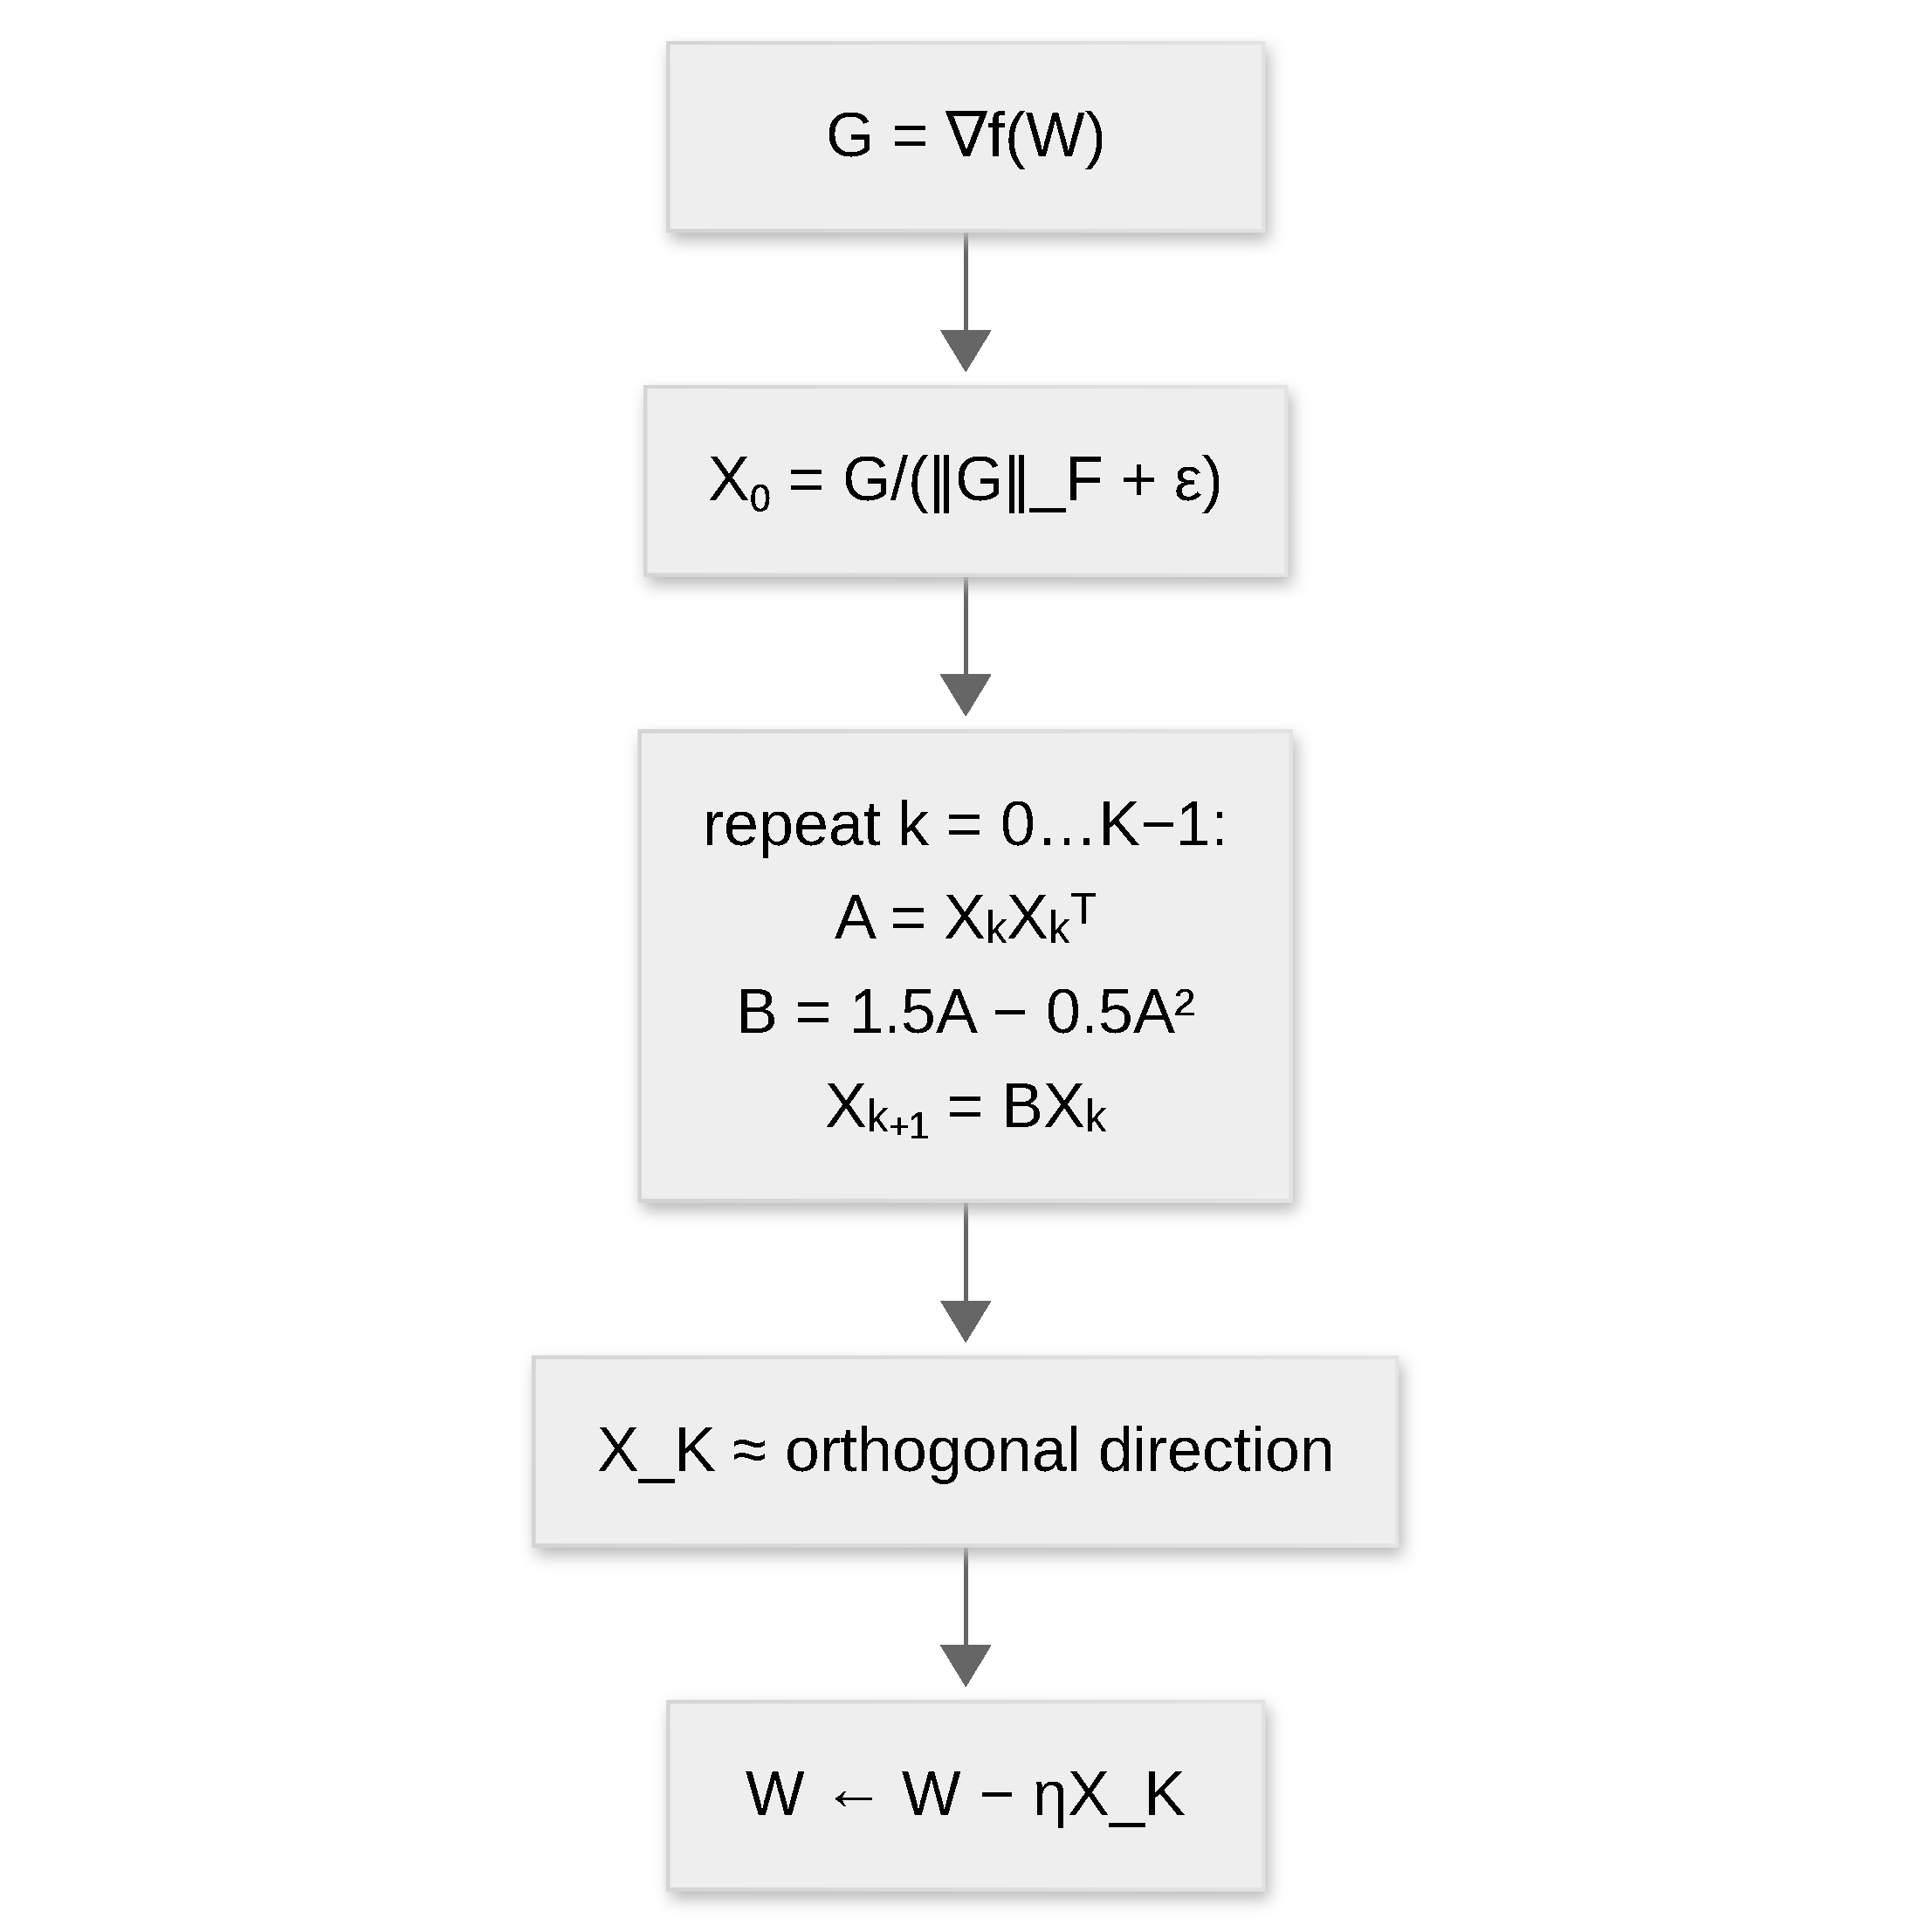
\includegraphics{figures/optimizers/muon.pdf}}
\caption{Step flow of Muon: Frobenius normalization followed by Newton-Schulz iterations that orthogonalize the update direction.}
\label{fig:opt-muon}
\end{figure}
Muon is an \textbf{orthogonality-oriented optimizer} that reshapes update geometry using Newton-Schulz polynomial iterations for orthogonalization. For a 2D parameter matrix $W$ with gradient $G_t$:
\begin{align}
X_0 &= \frac{G_t}{\|G_t\|_F + \epsilon} \quad\text{(normalized gradient)} \\
A_k &= X_k X_k^\top \quad\text{(Gramian)} \\
B_k &= b A_k + c A_k^2 \quad\text{(polynomial step, coefficients $b, c$ from Newton-Schulz)} \\
X_{k+1} &= a X_k + B_k X_k \quad\text{(iteration $k=0,1,\ldots,4$)} \\
W_{t+1} &= W_t - \eta X_K \quad\text{(update with orthogonalized direction)}
\end{align}
Muon performs 5 Newton-Schulz iterations to produce an approximately orthogonal direction, ensuring updates respect geometric constraints. The rationale: orthogonal updates preserve norms during training, avoiding the norm creep observed in momentum-based methods.

Following the hybrid recipe of \citet{shen_convergence_2025}, the orthogonalized update is reserved for hidden-layer weight matrices ($\mathtt{attention}$, $\mathtt{ffn}$ and other hidden-block groups). Embedding tables, learned positional encodings, output heads and every non-matrix parameter (biases, normalization scales, convolution kernels) are trained with decoupled AdamW instead of being skipped, using the group-level learning rate, weight decay, $\beta_1, \beta_2$ and $\epsilon$ settings exposed by the per-group configuration.

\begin{algorithm}[H]
\caption{Muon (Newton-Schulz Orthogonalization)}
\label{alg:muon}
\begin{algorithmic}[1]
\Require Initial parameters $\theta$, learning rate $\eta$, Newton-Schulz iters $K$
\Ensure Updated parameters $\theta_T$
\For{each parameter $P$}
    \If{$P$ is a hidden-layer 2D matrix $W$}
        \State $G \gets \nabla f(W)$ \Comment{Gradient}
        \State $X_0 \gets \frac{G}{\|G\|_F + \epsilon}$ \Comment{Normalize gradient by Frobenius norm}
        \For{$k = 0, 1, \ldots, K-1$}
            \State $A_k \gets X_k X_k^\top$ \Comment{Gramian (cost: $O(mn^2)$ or $O(m^2n)$ for tall/wide)}
            \State $B_k \gets (3/2) A_k - (1/2) A_k^2$ \Comment{Newton-Schulz coefficients}
            \State $X_{k+1} \gets B_k X_k$ \Comment{Polynomial step}
        \EndFor
        \State $W \gets W - \eta X_K$ \Comment{Update with orthogonalized direction}
    \Else
        \State $P \gets \operatorname{AdamW}(P, \nabla f(P); \eta, \beta_1, \beta_2, \epsilon, \lambda)$ \Comment{Hybrid fallback: embeddings, pos, heads, non-matrices}
    \EndIf
\EndFor
\Return $\theta_T$
\end{algorithmic}
\end{algorithm}

\paragraph{Cons.}
\begin{itemize}[leftmargin=*]
\item Several matrix multiplications per Newton-Schulz iteration; efficient custom kernels are required.
\item The orthogonalized construction is defined only for 2D matrices; the remaining parameter classes depend on the AdamW fallback and its per-group learning-rate calibration.
\end{itemize}

\paragraph{Pros.}
\begin{itemize}[leftmargin=*]
\item Orthogonalized updates preserve norms and avoid the norm creep of momentum-based methods.
\item Promising results on large-scale training with fundamentally better-conditioned update geometry.
\end{itemize}

\paragraph{Turbo-Muon (AOL-Preconditioned Orthogonalization).}
\begin{figure}[H]
\centering
\fitfigure{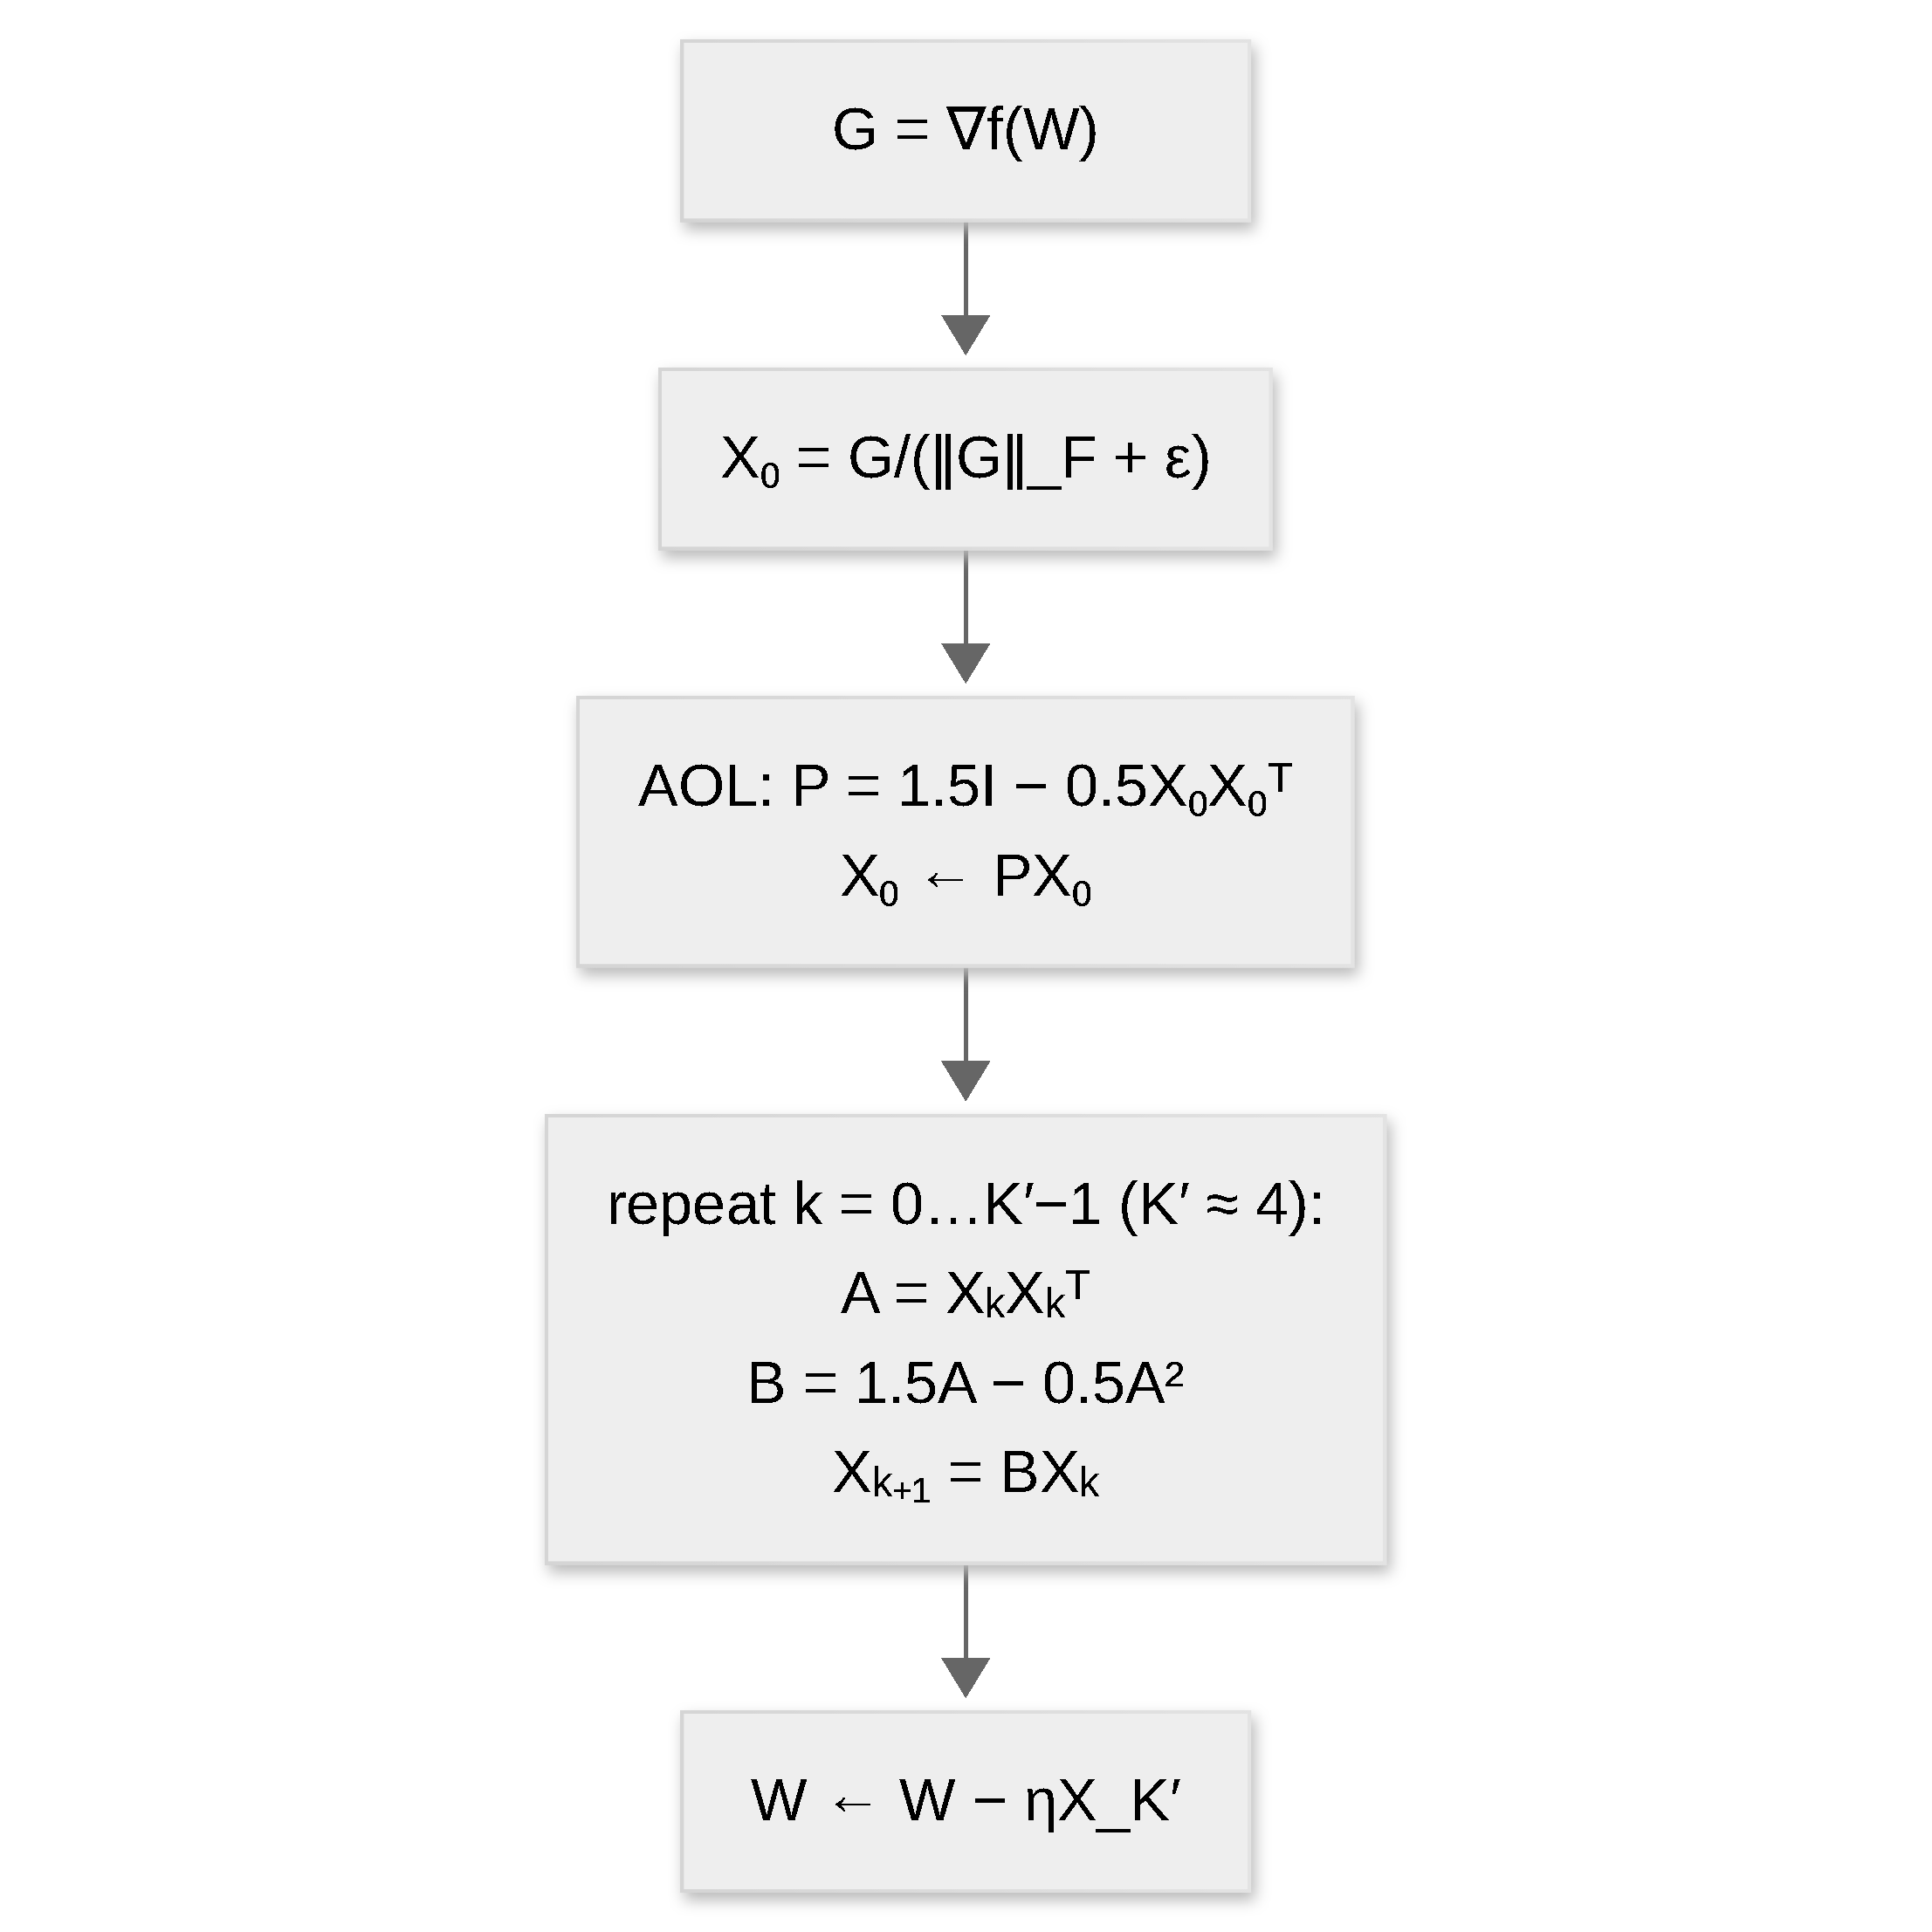
\includegraphics{figures/optimizers/turbo-muon.pdf}}
\caption{Step flow of Turbo-Muon: almost-orthogonal preconditioning (AOL) before the Newton-Schulz iterations, reducing their count.}
\label{fig:opt-turbo-muon}
\end{figure}
Turbo-Muon adds an \textbf{almost-orthogonal preconditioning} (AOL) step before the Newton-Schulz iterations. The preconditioner $P = 1.5I - 0.5X_0X_0^\top$ is applied to the normalized gradient, reducing the number of required orthogonalization steps to four while preserving the orthogonalized update geometry. It inherits Muon's hybrid routing: only hidden-layer 2D matrices are orthogonalized, while embedding tables, learned positional encodings, output heads and non-matrix parameters take decoupled AdamW updates.

\begin{algorithm}[H]
\caption{Turbo-Muon (AOL-Preconditioned Orthogonalization)}
\label{alg:turbo-muon}
\begin{algorithmic}[1]
\Require Initial parameters $\theta$, learning rate $\eta$, Newton-Schulz iters $K'$ (typically 4)
\Ensure Updated parameters $\theta_T$
\For{each parameter $P$}
    \If{$P$ is a hidden-layer 2D matrix $W$}
        \State $G \gets \nabla f(W)$ \Comment{Gradient}
        \State $X_0 \gets \frac{G}{\|G\|_F + \epsilon}$ \Comment{Normalize gradient}
        \State \textbf{AOL (Almost-Orthogonal preconditioner):} \Comment{Preconditioning step}
        \State $P \gets (1.5 I - 0.5 X_0 X_0^\top)$ \Comment{Preconditioning matrix}
        \State $X_0 \gets P X_0$ \Comment{Preconditioned start}
        \For{$k = 0, 1, \ldots, K'-1$}
            \State $A_k \gets X_k X_k^\top$
            \State $B_k \gets (3/2) A_k - (1/2) A_k^2$
            \State $X_{k+1} \gets B_k X_k$ \Comment{Reduced iterations due to AOL preconditioning}
        \EndFor
        \State $W \gets W - \eta X_{K'}$ \Comment{Update with preconditioned orthogonalized direction}
    \Else
        \State $P \gets \operatorname{AdamW}(P, \nabla f(P); \eta, \beta_1, \beta_2, \epsilon, \lambda)$ \Comment{Hybrid fallback: embeddings, pos, heads, non-matrices}
    \EndIf
\EndFor
\Return $\theta_T$
\end{algorithmic}
\end{algorithm}

\paragraph{Cons.}
\begin{itemize}[leftmargin=*]
\item Still compute-heavy; AOL adds a preconditioning matrix multiplication.
\item Requires the same custom-kernel support as Muon, and shares its dependence on the AdamW fallback for non-hidden parameter classes.
\end{itemize}

\paragraph{Pros.}
\begin{itemize}[leftmargin=*]
\item AOL reduces the Newton-Schulz iteration count (typically five to four).
\item Retains orthogonalized update geometry at lower iteration cost.
\end{itemize}

\paragraph{AF-Muon (AdamW-Free Tied-Embedding Muon).}
\begin{figure}[H]
\centering
\fitfigure{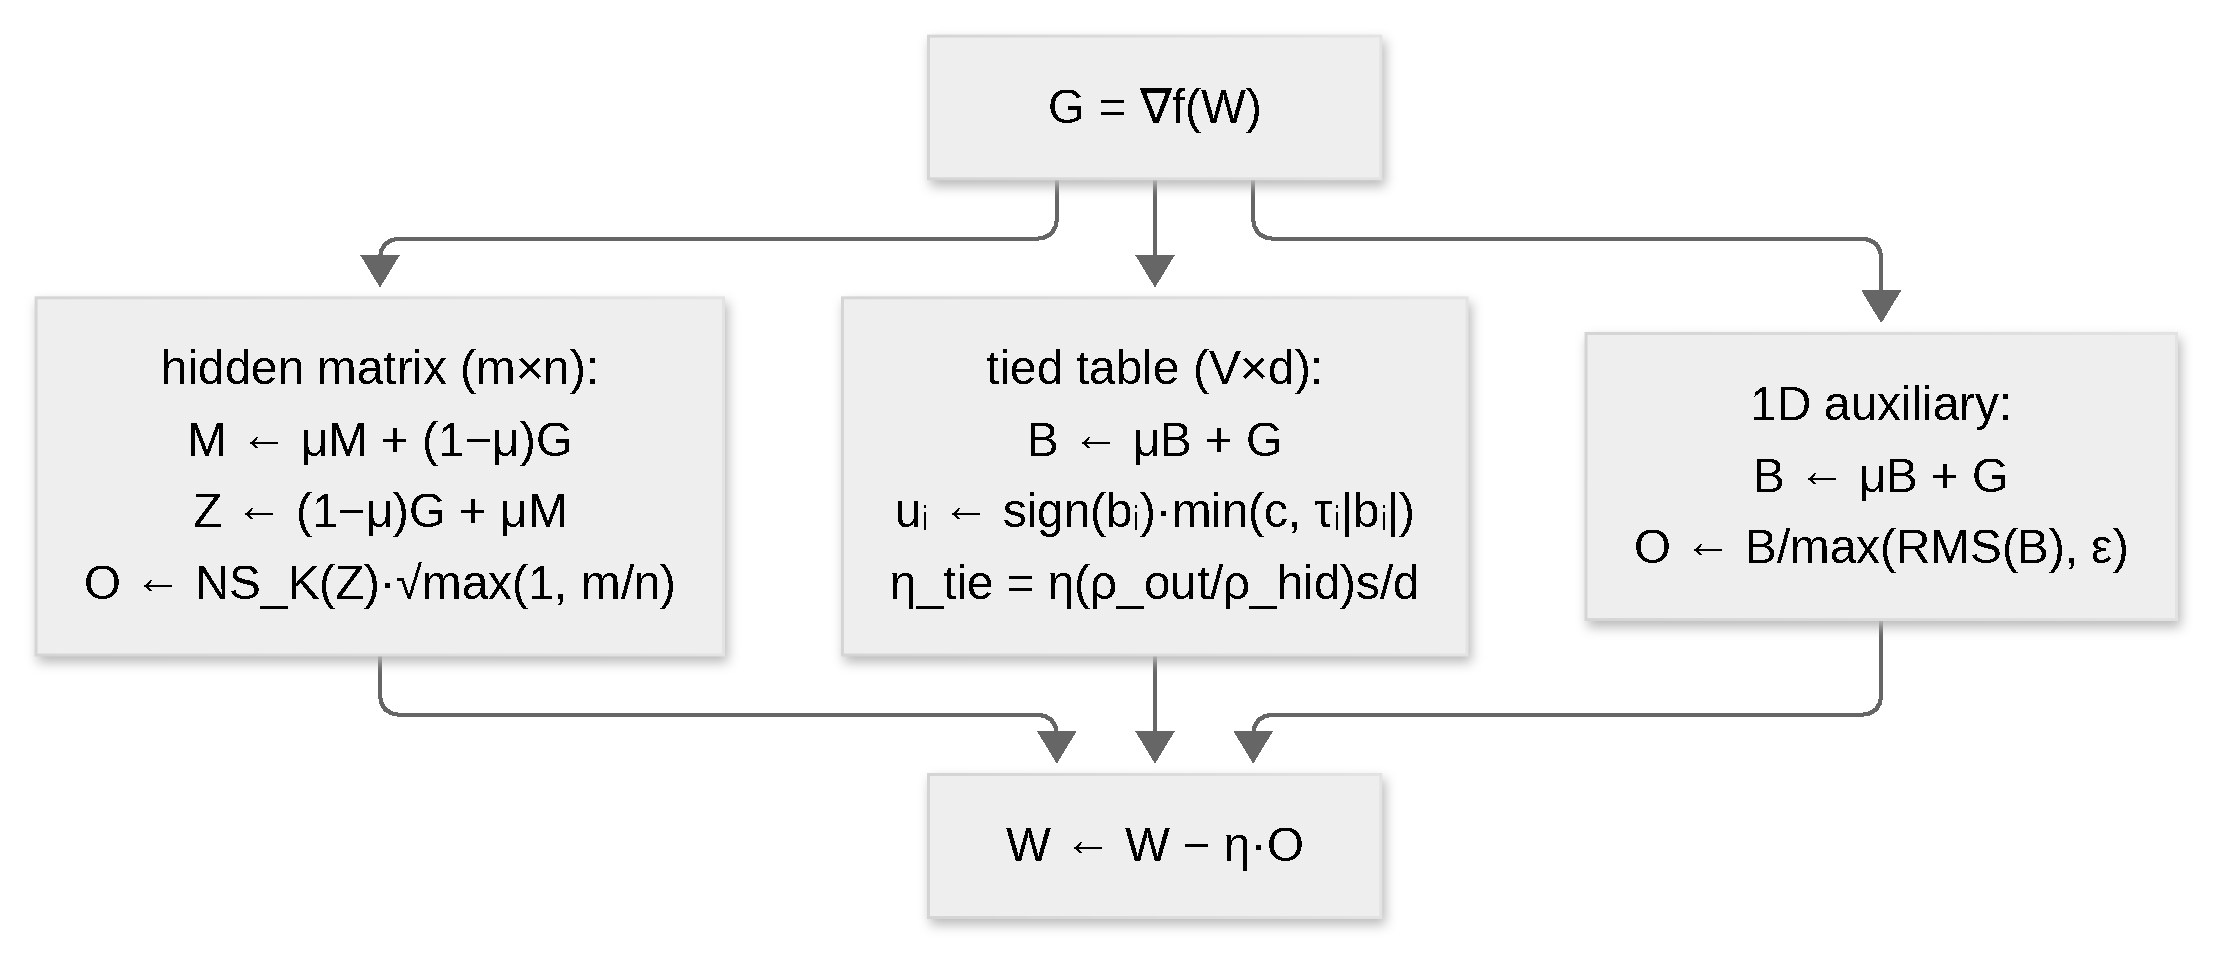
\includegraphics{figures/optimizers/af-muon.pdf}}
\caption{Step flow of AF-Muon: Muon's spectral update for hidden matrices, a support-aware finite-cap clipped-row LMO for the tied vocabulary table, and RMS-normalized updates for one-dimensional auxiliary parameters, all with a single first-moment buffer.}
\label{fig:opt-af-muon}
\end{figure}
AF-Muon is an \textbf{AdamW-free extension of Muon} that removes the auxiliary AdamW fallback of the Hybrid Muon recipe by giving every parameter class its own norm-constrained geometry. Hidden matrices keep the spectral update with a Nesterov signal; the vocabulary table, which simultaneously receives sparse input-lookup and dense output-softmax gradients, is updated row by row with a \emph{support-aware finite-cap linear minimization oracle}; one-dimensional auxiliary tensors receive an RMS-normalized update. No parameter class carries second-moment state, so a single first-moment buffer per parameter replaces the AdamW state of the hybrid recipe, which the authors report as roughly 20\% less optimizer-state memory at matched training.

For the tied table $W \in \mathbb{R}^{V \times d}$ with momentum row $b_i$, the oracle solves the row problem
\begin{align}
u_i &= \operatorname{sign}(b_i) \odot \min\left(c\,\mathbf{1},\ \tau_i\,|b_i|\right), \\
\|u_i\|_2^2 &= \min\left(d,\ c^2\,\bigl|\operatorname{supp}(b_i)\bigr|\right),
\end{align}
where the per-row scale $\tau_i$ is obtained by bisection in FP32 over complete-row chunks. Rows whose support cannot fill the row-$\ell_2$ radius saturate every useful coordinate at the cap $c$, so sparse lookup rows are handled without inflating absent coordinates. The cap interpolates between two known endpoints: $c = 1$ recovers the SCION-style Sign update and $c \geq \sqrt{d}$ reduces to a row-RMS update. The tied step size is $\eta_{tie} = \eta_M (\rho_{out}/\rho_{hid})\, s / d$; the paper's main setting is $c = 3$ and $s = 0.5$ with $\rho_{out}/\rho_{hid} = 60$, and its diagnostics report the finite cap active on under 0.3\% of coordinates while affecting most rows.

\begin{algorithm}[H]
\caption{AF-Muon (AdamW-Free Tied-Embedding Muon)}
\label{alg:af-muon}
\begin{algorithmic}[1]
\Require Initial parameters $\theta$, matrix LR $\eta_M$, vector LR $\eta_{vec}$, momentum $\mu$, matrix weight decay $\lambda_M$, tied scale $s$, cap $c$, radii $\rho_{out}, \rho_{hid}$, Newton-Schulz iters $K$
\Ensure Updated parameters $\theta_T$
\For{each parameter tensor $W$ with gradient $G_t$}
    \If{$W$ is a hidden matrix in $\mathbb{R}^{m \times n}$}
        \State $M_t \gets \mu M_{t-1} + (1-\mu) G_t$ \Comment{First moment}
        \State $Z_t \gets (1-\mu) G_t + \mu M_t$ \Comment{Nesterov signal}
        \State $O_t \gets \mathrm{NS}_K(Z_t)\sqrt{\max(1, m/n)}$ \Comment{Spectral update}
        \State $W_t \gets (1 - \eta_M \lambda_M) W_{t-1} - \eta_M O_t$
    \ElsIf{$W \in \mathbb{R}^{V \times d}$ is the tied vocabulary table}
        \State $B_t \gets \mu B_{t-1} + G_t$ \Comment{Unnormalized first moment}
        \State $\eta_{tie,t} \gets \eta_M (\rho_{out}/\rho_{hid}) s / d$
        \For{each row $i = 1, \ldots, V$}
            \State $u_i \gets L_c\bigl(\mathrm{row}_i(B_t)\bigr)$ \Comment{Capped-row LMO}
        \EndFor
        \State $W_t \gets W_{t-1} - \eta_{tie,t} U$
    \Else
        \State $B_t \gets \mu B_{t-1} + G_t$ \Comment{$1$D auxiliary tensor}
        \State $O_t \gets B_t / \max(\mathrm{RMS}(B_t), \epsilon)$
        \State $W_t \gets W_{t-1} - \eta_{vec} O_t$
    \EndIf
\EndFor
\Return $\theta_T$
\end{algorithmic}
\end{algorithm}

\paragraph{Cons.}
\begin{itemize}[leftmargin=*]
\item Every parameter must be assigned an explicit role (matrix, tied table, or vector); an untied output head or an extra embedding table is not a tied-table block.
\item The tied-table oracle requires a per-row bisection with complete-row chunking; the paper reports roughly 1\% median step-time overhead at matched training.
\item The tied-table claim is established for tied-vocabulary models; frontier-scale pretraining and universal endpoint superiority are not claimed.
\end{itemize}

\paragraph{Pros.}
\begin{itemize}[leftmargin=*]
\item AdamW-free: one first-moment buffer per parameter and no second-moment state, reported as roughly 20\% less optimizer-state memory than Hybrid Muon.
\item The finite cap preserves within-row magnitudes while bounding coordinate concentration, and recovers Sign ($c=1$) and row-RMS ($c \geq \sqrt{d}$) as limit cases.
\item Improves mean validation loss and perplexity over both Hybrid Muon and a SCION-style Sign endpoint across nine tied-token settings spanning text, image-token, protein, MoE, and encoder-decoder models.
\end{itemize}

\paragraph{AdaMuon (Adaptive Muon).}
AdaMuon is an \textbf{adaptive extension of Muon} that keeps the spectral (polar) update while adding coordinate-wise variance normalization. Muon orthogonalizes the momentum matrix into a direction-only update, which removes anisotropic scaling but assigns the same magnitude to every coordinate; AdaMuon addresses the resulting mismatch between noisy and informative coordinates by tracking the element-wise variance of the \emph{orthogonalized} direction rather than of the raw gradient or of the momentum. Because the polar factor is globally scale-invariant, the sign transform applied before orthogonalization preserves the update direction while stabilizing its element-wise magnitudes; the paper proves that $\operatorname{sign}$ is the unique element-wise map that is scale-free, sign-consistent, odd and bounded (Theorem~1). The second-moment estimate therefore sees a stable signal, and its variance-normalized version is rescaled to an RMS of $0.2$, matching Adam's empirical update scale so that existing learning-rate schedules are reused without tuning.

For a weight $W_t \in \mathbb{R}^{n \times m}$, momentum buffer $M_t$, momentum $\beta$, Newton--Schulz steps $T$ and small constant $\varepsilon$:
\begin{align}
M_t &= \beta M_{t-1} + G_t, \\
O_t &= \operatorname{NewtonSchulz}\bigl(\operatorname{sign}(M_t), T\bigr), \\
V_t &= \beta V_{t-1} + (1-\beta)\, O_t \odot O_t, \\
\widehat{O}_t &= O_t \oslash \bigl(\sqrt{V_t} + \varepsilon \mathbf{1}\bigr), \\
\gamma_t &= \frac{0.2\sqrt{mn}}{\|\widehat{O}_t\|_F}, \\
W_{t+1} &= W_t - \eta\bigl(\gamma_t \widehat{O}_t + \lambda W_t\bigr).
\end{align}
The Newton--Schulz map uses $X_0 = \operatorname{sign}(M_t)/\|\operatorname{sign}(M_t)\|_F$ and the cubic iteration $X_k = aX_{k-1} + b(X_{k-1}X_{k-1}^{\mathsf T})X_{k-1} + c(X_{k-1}X_{k-1}^{\mathsf T})^2X_{k-1}$ with $(a,b,c) = (3.4445, -4.7750, 2.0315)$ and $T = 5$. No bias correction is applied to either moment: a constant factor in $V_t$ is cancelled exactly by $\gamma_t \propto \sqrt{c}$, and a constant factor in $M_t$ is removed by the polar map, $\operatorname{polar}(cM) = \operatorname{polar}(M)$.

\begin{algorithm}[H]
\caption{AdaMuon (Adaptive Muon)}
\label{alg:ada-muon}
\begin{algorithmic}[1]
\Require Initial weights $W_0 \in \mathbb{R}^{n \times m}$, learning rate $\eta$, weight decay $\lambda$, momentum $\beta$, Newton--Schulz steps $T$, small constant $\varepsilon$
\Ensure Updated weights $W_T$
\State $M_0 \gets \mathbf{0}$, $V_0 \gets \mathbf{0}$
\For{each iteration $t = 1, 2, \ldots$}
    \State $G_t \gets \nabla_{W_t}\mathcal{L}(W_t)$
    \State $M_t \gets \beta M_{t-1} + G_t$
    \State $O_t \gets \operatorname{NewtonSchulz}(\operatorname{sign}(M_t), T)$
    \State $V_t \gets \beta V_{t-1} + (1-\beta)\, O_t \odot O_t$
    \State $\widehat{O}_t \gets O_t \oslash (\sqrt{V_t} + \varepsilon\mathbf{1})$
    \State $\gamma_t \gets 0.2\sqrt{mn}/\|\widehat{O}_t\|_F$
    \State $W_{t+1} \gets W_t - \eta(\gamma_t \widehat{O}_t + \lambda W_t)$
\EndFor
\Return $W_T$
\end{algorithmic}
\end{algorithm}

\paragraph{Cons.}
\begin{itemize}[leftmargin=*]
\item One additional second-moment buffer per matrix parameter (two buffers versus Muon's single first-moment buffer), plus per-step element-wise EMA, square-root and normalization work on the update.
\item The update is defined for two-dimensional parameters; one-dimensional parameters (biases, norm scales) require an auxiliary optimizer in the paper's recipe.
\item The RMS target ($0.2$) is a fixed constant rather than a learned quantity, so the method assumes Adam-like update scales when reusing existing schedules.
\end{itemize}

\paragraph{Pros.}
\begin{itemize}[leftmargin=*]
\item No new hyperparameters: the second-moment EMA reuses Muon's momentum coefficient $\beta$, and the paper reports low sensitivity across $\beta \in [0.8, 0.99]$.
\item The sign transform makes the variance estimate stable enough to normalize, and the RMS alignment cancels any constant bias in $V_t$, so no bias correction is needed for either moment.
\item RMS alignment matches Adam's update scale, allowing direct reuse of learning-rate schedules; the authors report up to roughly 40\% training-efficiency gains over AdamW and consistent wins over Muon on GPT-2 (125M--1.5B) and Qwen2.5 (1.5B, 7B).
\end{itemize}

\paragraph{Dion3 (Fractional Gram-Newton-Schulz Orthogonalization).}
Dion3~\citep{amsel_dion3_2026} is a \textbf{revision of Muon} that reduces the cost of the orthogonalization step at the algorithmic level. It replaces standard Newton--Schulz with \emph{Gram Newton--Schulz}, a mathematically equivalent iteration that runs on the small symmetric Gram matrix $XX^{\mathsf T}$, and it orthogonalizes only a fraction $f \in (0,1]$ of the momentum rows at each step, updating only those rows of the weight matrix. \emph{Error feedback} decays only the selected rows of the momentum buffer, so rows that were not selected keep accumulating and are eventually chosen. At $f = 1$ the update reduces to Muon in exact arithmetic (or to NorMuon with the optional row-wise normalization). For a weight $W \in \mathbb{R}^{n \times m}$ (operating on the smaller dimension, $n \le m$), fraction $f$, $k = \lceil f n \rceil$, momentum $\mu$, learning rate $\eta$ and weight decay $\lambda$:
\begin{align}
M_t &= M_{t-1} + G_t \quad\text{(momentum accumulation; damping deferred)} \\
S_t &= \operatorname{topk}_{i}\bigl(\lVert M_{t,i,:}\rVert_1,\ k\bigr) \quad\text{(select the } k \text{ largest rows)} \\
O_t &= \operatorname{GramNS}\bigl(M_t[S_t,:]\bigr) \quad\text{(orthogonalize the } k \times m \text{ submatrix)} \\
W_t &= (1 - \eta\lambda)\, W_{t-1}, \qquad W_t[S_t,:] \gets W_t[S_t,:] - \eta\, O_t \\
M_t[S_t,:] &\gets \mu\, M_t[S_t,:] \quad\text{(error feedback: decay only selected rows)}
\end{align}
Gram Newton--Schulz normalizes $X \gets M_t[S_t,:]/(\lVert M_t[S_t,:]\rVert_F + \epsilon)$ with $\epsilon = 10^{-7}$, casts to \texttt{float16}, forms $R_0 = X X^{\mathsf T}$ and $Q_0 = I$, and runs $T$ iterations
\begin{align}
Z_t &= b_t R_{t-1} + c_t R_{t-1}^2, &
Q_t &= Q_{t-1} Z_t + a_t Q_{t-1}, \\
(RZ)_t &= R_{t-1} Z_t + a_t R_{t-1}, &
R_t &= Z_t (RZ)_t + a_t (RZ)_t,
\end{align}
returning $Q_T X$. A \emph{restart} after iteration~2 ($X \gets Q_2 X$, $R_2 \gets X X^{\mathsf T}$, $Q_2 \gets I$) removes the spurious negative eigenvalues that half precision introduces in the Gram matrix; the coefficients $(a_t,b_t,c_t)$ are the Polar Express five-step triples~\citep{amsel_polar_express_2026}. The cost falls from $T(3\alpha+1)n^3$ FLOPs for standard Newton--Schulz to $(4T+3\alpha-3)n^3$ for Gram Newton--Schulz ($\alpha = m/n$), and selecting $k = \lceil f n \rceil$ rows both shrinks the iteration and raises the aspect ratio by $1/f$. The optional NorMuon flavor adds a row-wise second moment $v_i \gets \beta_2 v_i + (1-\beta_2)\,\operatorname{mean}_j(O_{ij}^2)$ for $i \in S$, rescales $\tilde O_{ij} = O_{ij}/(\sqrt{v_i}+\epsilon)$, and renormalizes $\tilde O \gets \tilde O\,\lVert O\rVert_F/\lVert\tilde O\rVert_F$ in \texttt{float32} before the update.

\begin{algorithm}[H]
\caption{Dion3 (Fractional Orthogonalization with Error Feedback)}
\label{alg:dion3}
\begin{algorithmic}[1]
\Require Matrices $W$, learning rate $\eta$, momentum $\mu$, fraction $f$, Gram Newton--Schulz steps $T$, $\epsilon$, weight decay $\lambda$
\Ensure Updated matrices $W_T$
\For{each 2D parameter matrix $W$ with gradient $G$}
    \State $M \gets M + G$ \Comment{Momentum accumulation}
    \State $S \gets$ indices of the $k = \lceil f n \rceil$ rows of $M$ with largest $\ell_1$ norm \Comment{Selection}
    \State $O \gets \operatorname{GramNS}_T(M[S,:])$ \Comment{Orthogonalize the selected submatrix}
    \If{NorMuon}
        \State $v_i \gets \beta_2 v_i + (1-\beta_2)\operatorname{mean}_j(O_{ij}^2)$ for $i \in S$
        \State $\tilde O_{ij} \gets O_{ij}/(\sqrt{v_i}+\epsilon)$; \quad $\tilde O \gets \tilde O\,\lVert O\rVert_F/\lVert\tilde O\rVert_F$
    \EndIf
    \State $W \gets (1 - \eta\lambda) W$ \Comment{Weight decay on all rows}
    \State $W[S,:] \gets W[S,:] - \eta\,\tilde O$ \Comment{Update selected rows only}
    \State $M[S,:] \gets \mu\, M[S,:]$ \Comment{Error feedback}
\EndFor
\Return $W_T$
\end{algorithmic}
\end{algorithm}

\paragraph{Cons.}
\begin{itemize}[leftmargin=*]
\item Each step updates only a fraction of the rows, so the optimization trajectory differs from Muon; the paper reports the change is benign (Section~8.1 of the Dion3 report).
\item Row selection and error feedback add top-$k$ bookkeeping and a row-wise momentum decay per step.
\item The largest wall-clock gains in the paper come from symmetric GEMM kernels and megabatched communication, which are hardware- and cluster-specific; only the algorithmic reduction and the single first-moment buffer apply here.
\end{itemize}

\paragraph{Pros.}
\begin{itemize}[leftmargin=*]
\item Gram Newton--Schulz is mathematically equivalent to Newton--Schulz and cuts orthogonalization FLOPs by about 55\% at typical transformer aspect ratios with five iterations.
\item Fractional row selection reduces the orthogonalized submatrix to $k \times m$ and raises its aspect ratio by $1/f$, compounding the Gram savings; the paper reports up to $6\times$ faster optimizer steps at matched loss.
\item At $f = 1$ the update reduces to Muon (or NorMuon), and a single momentum buffer per matrix parameter suffices; error feedback lets ignored rows participate eventually.
\end{itemize}

\paragraph{ROOT (Robust Orthogonalized Optimizer).}
\begin{figure}[H]
\centering
\fitfigure{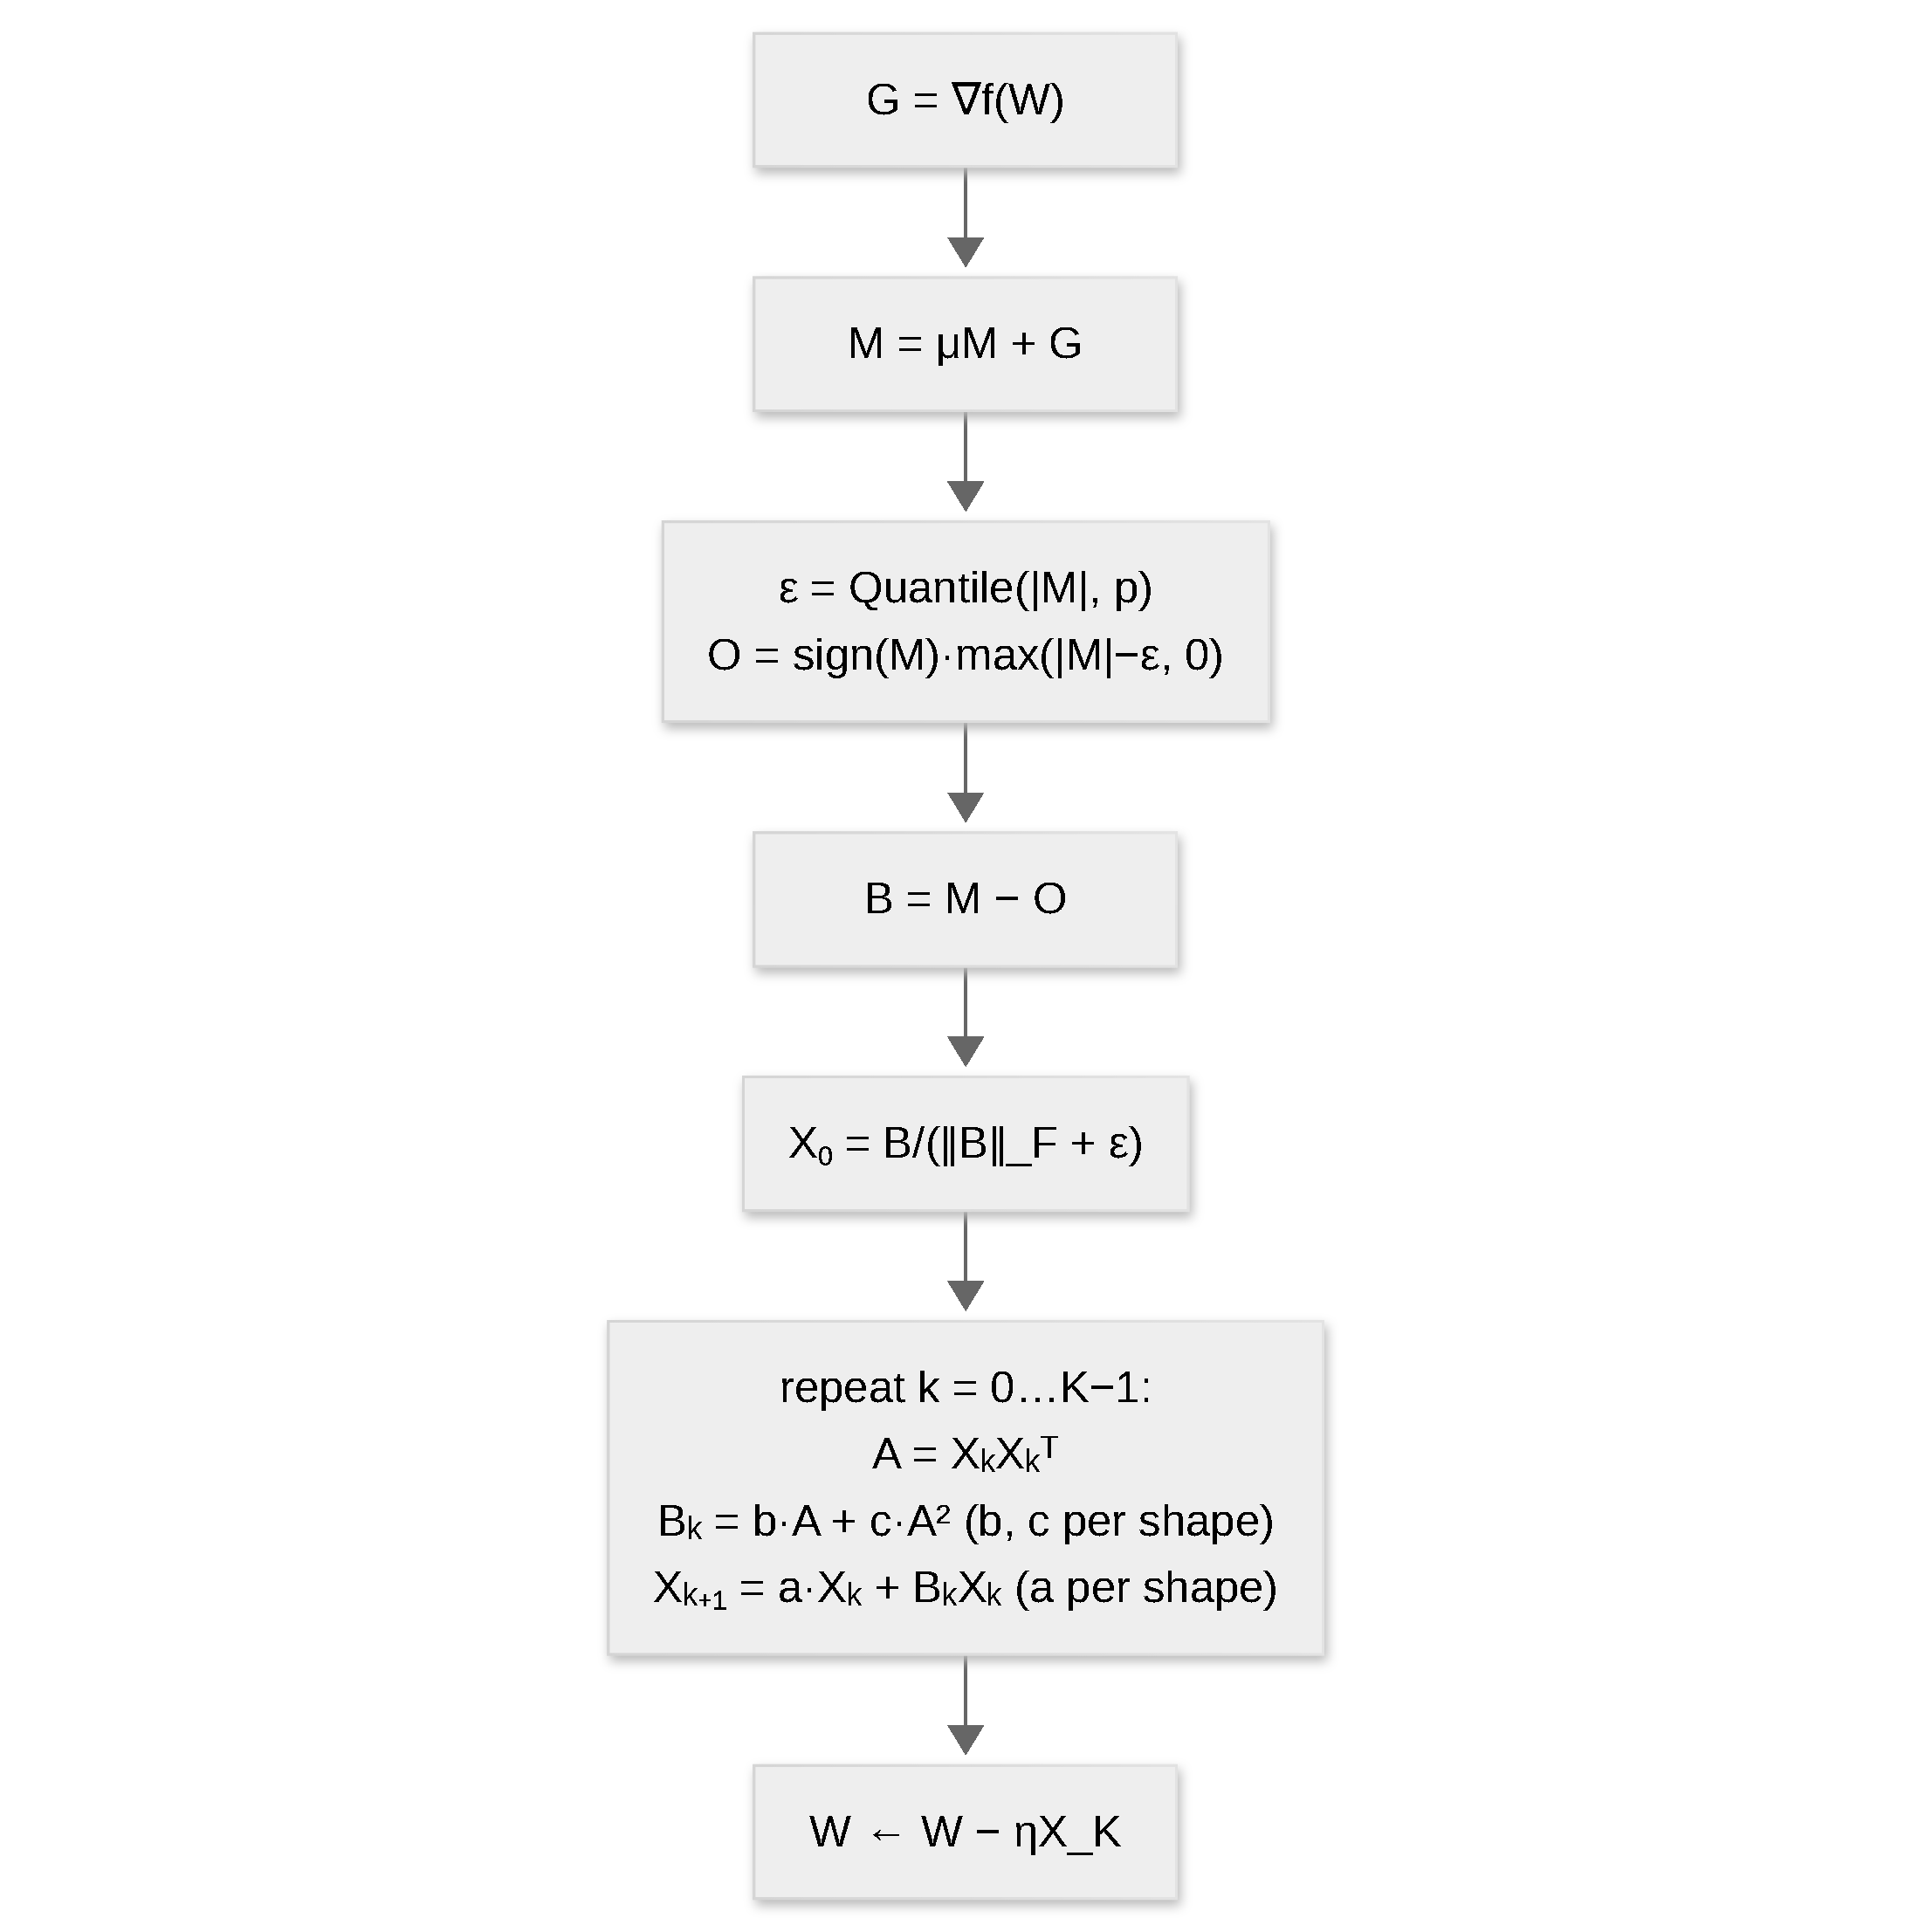
\includegraphics{figures/optimizers/root.pdf}}
\caption{Step flow of ROOT: momentum accumulation, soft-threshold outlier separation, and shape-calibrated Newton--Schulz orthogonalization.}
\label{fig:opt-root}
\end{figure}
ROOT~\citep{he_root_2025} is a \textbf{robustness-oriented revision of Muon} that attacks two fragilities of the fixed-coefficient Newton--Schulz pipeline. First, the universal coefficients $(a,b,c)=(3.4445,-4.7750,2.0315)$ are calibrated for an ``average'' matrix shape and lose precision exactly on square and near-square layers: the orthogonalization MSE ranges from $0.0499$ at $2048\times2048$ to $0.0003$ at $2048\times16384$ in Table~1 of the paper. ROOT replaces them with per-shape coefficients $\{a^{(m,n)}, b^{(m,n)}, c^{(m,n)}\}$ calibrated offline over momentum singular-value distributions (Mixed 1:3 real-to-random calibration), a scheme the authors call \emph{AdaNewton}. Second, heavy-tailed gradient components distort the Frobenius normalization required by Newton--Schulz and are amplified by the polynomial iteration; ROOT models the momentum as $M_t = B_t + O_t$ and solves a proximal L1 problem whose closed-form solution is soft-thresholding. Only the robust base component $B_t$ is orthogonalized; the sparse outlier component $O_t$ is discarded. For a hidden-layer weight matrix $W \in \mathbb{R}^{m\times n}$, momentum $\mu$, learning rate $\eta$, percentile $p$ and iteration count $K$:
\begin{align}
M_t &= \mu M_{t-1} + \nabla \mathcal{L}(\theta_{t-1}) \quad\text{(momentum, Eq. 1)} \\
\varepsilon_t &= \operatorname{Quantile}(|M_t|, p) \quad\text{(dynamic threshold, } p=0.90 \text{ default)} \\
O_t &= \mathcal{T}_{\varepsilon_t}[M_t], \quad \mathcal{T}_\varepsilon[x]_i = \operatorname{sign}(x_i)\max(|x_i|-\varepsilon, 0) \quad\text{(soft-threshold, Eqs. 7--10)} \\
B_t &= M_t - O_t \quad\text{(clipped robust component, Eq. 9)} \\
X_0 &= \frac{B_t}{\lVert B_t\rVert_F}, \qquad X_k = a^{(m,n)}X_{k-1} + b^{(m,n)}X_{k-1}(X_{k-1}^\top X_{k-1}) + c^{(m,n)}X_{k-1}(X_{k-1}^\top X_{k-1})^2 \\
\theta_t &= \theta_{t-1} - \eta X_K \quad\text{(update, } K=5\text{)}
\end{align}

\begin{table}[H]
\centering
\caption{AdaNewton coefficients from Table~1 of \citet{he_root_2025} (Mixed 1:3 calibration). Shapes outside the table fall back to Muon's fixed $(3.4445,-4.7750,2.0315)$.}
\label{tab:root-coefficients}
\small
\begin{tabular}{rrrrrr}
\toprule
$m$ & $n$ & $a^{(m,n)}$ & $b^{(m,n)}$ & $c^{(m,n)}$ & MSE \\
\midrule
2048 & 2048 & 3.3334 & $-4.2591$ & 1.7791 & 0.0352 \\
4096 & 4096 & 3.3732 & $-4.6134$ & 2.0576 & 0.0470 \\
8192 & 8192 & 3.3886 & $-4.9026$ & 2.3105 & 0.0587 \\
3072 & 2048 & 2.9091 & $-3.8108$ & 1.8600 & 0.0024 \\
4096 & 2048 & 2.7739 & $-3.4911$ & 1.6992 & 0.0010 \\
8192 & 2048 & 2.5925 & $-3.0010$ & 1.4138 & 0.0003 \\
16384 & 2048 & 2.7045 & $-3.2335$ & 1.5336 & 0.0003 \\
\bottomrule
\end{tabular}
\end{table}

\begin{algorithm}[H]
\caption{ROOT (Robust Orthogonalized Optimizer)}
\label{alg:root}
\begin{algorithmic}[1]
\Require Initial parameters $\theta$, learning rate $\eta$, momentum $\mu$, percentile $p$, Newton--Schulz iters $K$
\Ensure Updated parameters $\theta_T$
\For{each parameter $P$}
    \If{$P$ is a hidden-layer 2D matrix $W$}
        \State $G \gets \nabla f(W)$ \Comment{Gradient}
        \State $M \gets \mu M + G$ \Comment{Momentum accumulation}
        \State $\varepsilon \gets \operatorname{Quantile}(|M|, p)$ \Comment{Dynamic threshold}
        \State $O \gets \operatorname{sign}(M)\max(|M|-\varepsilon, 0)$ \Comment{Outlier separation (soft-threshold)}
        \State $B \gets M - O$ \Comment{Clipped robust component}
        \State $X_0 \gets \frac{B}{\|B\|_F + \epsilon}$ \Comment{Normalize by Frobenius norm}
        \For{$k = 0, 1, \ldots, K-1$}
            \State $A_k \gets X_k X_k^\top$ \Comment{Gramian}
            \State $B_k \gets b^{(m,n)} A_k + c^{(m,n)} A_k^2$ \Comment{Shape-calibrated coefficients}
            \State $X_{k+1} \gets a^{(m,n)} X_k + B_k X_k$ \Comment{Polynomial step}
        \EndFor
        \State $W \gets W - \eta X_K$ \Comment{Update with orthogonalized direction}
    \Else
        \State $P \gets \operatorname{AdamW}(P, \nabla f(P); \eta, \beta_1, \beta_2, \epsilon, \lambda)$ \Comment{Hybrid fallback: embeddings, pos, heads, non-matrices}
    \EndIf
\EndFor
\Return $\theta_T$
\end{algorithmic}
\end{algorithm}

Following the hybrid recipe of Muon, only hidden-layer 2-D matrices take the ROOT path; embedding tables, learned positional encodings, output heads and every non-matrix parameter are trained with decoupled AdamW using the group-level learning rate, weight decay, $\beta_1, \beta_2$ and $\epsilon$ settings. The paper's LLM runs apply a $0.2$ update-RMS scaling factor following Moonlight; this implementation lets the per-group learning rates absorb that calibration, so no scale constant is applied. Shapes absent from Table~\ref{tab:root-coefficients} fall back to Muon's fixed coefficients, and the dynamic quantile costs an additional sort of $|M_t|$ per matrix per step.

\paragraph{Cons.}
\begin{itemize}[leftmargin=*]
\item The percentile threshold requires an $O(N\log N)$ sort of the momentum matrix at every step, on top of the Newton--Schulz matmuls.
\item The calibrated coefficient table covers seven shapes only; every other shape falls back to Muon's fixed coefficients.
\item Outliers are discarded rather than shrunk, so an extremely noisy gradient can also lose informative signal; the paper's ablation shows the trade-off is governed by the percentile (0.85 truncates too much, 0.99 too little).
\end{itemize}

\paragraph{Pros.}
\begin{itemize}[leftmargin=*]
\item Dimension-invariant orthogonalization precision: shape-calibrated coefficients remove the precision cliff that fixed coefficients show on square and near-square layers.
\item Outlier-robust without retuning the Muon recipe; the paper reports lower loss and a better zero-shot average than Muon and AdamW at 1B scale (60.12 vs 59.59 vs 59.05) and gains on ViT/CIFAR-10.
\item Same single momentum buffer per matrix parameter as Muon, and the \texttt{softthresh}/\texttt{ada\_newton} toggles expose the paper's ablations directly.
\end{itemize}

\paragraph{Muon² (Second-Moment Preconditioned Orthogonalization).}
Muon$^2$~\citep{liu_muon2_2026} generalizes Muon by preconditioning the momentum with an
\textbf{Adam-style second-moment EMA before the Newton--Schulz orthogonalization}. The
paper shows that the practical bottleneck of Muon's polar approximation is the
ill-conditioned momentum matrix (early-training spectra span $10^{-4}$--$1$ with roughly
half the singular values in the NS ``dead zone''); dividing by $\sqrt{V_t}$ tightens the
spectrum, so every NS step aligns better with the true orthogonalized update (cosine
similarity $0.916$ at $K{=}3$ vs Muon's $0.931$ at $K{=}5$, rising to $0.975$ at
$K{=}5$). For a hidden-layer weight matrix $W \in \mathbb{R}^{n \times m}$ with learning
rate $\eta$:
\begin{align}
M_t &= \beta_1 M_{t-1} + (1-\beta_1) G_t && \text{(momentum EMA, Eq.~2)} \\
V_t &= \beta_2 V_{t-1} + (1-\beta_2)\, (G_t \odot G_t) && \text{(second-moment EMA, Eq.~3)} \\
\widetilde{M}_t &= M_t \oslash \big(\sqrt{V_t} + \epsilon \mathbf{1}\big) && \text{(preconditioning, Eq.~4)} \\
X_0 &= \frac{\widetilde{M}_t}{\|\widetilde{M}_t\|_F + \epsilon}, \qquad
X_{k+1} = aX_k + b\, X_k X_k^\top X_k + c\, X_k (X_k X_k^\top)^2 X_k && \text{(NS, Eq.~5)} \\
W_{t+1} &= W_t - \eta \sqrt{m/n}\, X_K && \text{(update, Eq.~6)}
\end{align}
with the same quintic coefficients $(a,b,c)=(3.4445,-4.7750,2.0315)$ as Muon and the
$\sqrt{m/n}$ learning-rate factor proposed by Bernstein (2025). The memory-efficient
variant \textbf{Muon$^2$-F} replaces $V_t$ with Adafactor-style row/column statistics:
\begin{align}
r_t &= \beta_2 r_{t-1} + (1-\beta_2)\,\mathrm{sum}_{\mathrm{col}}(G_t \odot G_t), \qquad
c_t = \beta_2 c_{t-1} + (1-\beta_2)\,\mathrm{sum}_{\mathrm{row}}(G_t \odot G_t), \\
\widehat{V}_t &= \frac{r_t\, c_t^\top}{\mathrm{sum}(r_t)},
\end{align}
keeping memory within $\sim$0.3\% of Muon at 7B scale (47.53 vs 47.29 GB) while retaining
most of Muon$^2$'s benefit. Across GPT, LLaMA and Mixture-of-Experts pre-training up to
13B parameters, Muon$^2$ outperforms Muon at equal NS iterations and matches it with
$K{=}3$ instead of $5$ (a 40\% reduction), saving up to a quarter of training time at
equal loss.

\begin{algorithm}[H]
\caption{Muon² (Second-Moment Preconditioned Orthogonalization)}
\label{alg:muon2}
\begin{algorithmic}[1]
\Require Initial parameters $\theta$, learning rate $\eta$, $\beta_1, \beta_2$, NS iters $K$, preconditioner $\epsilon$
\Ensure Updated parameters $\theta_T$
\For{each parameter $P$}
    \If{$P$ is a hidden-layer 2D matrix $W \in \mathbb{R}^{n\times m}$}
        \State $G \gets \nabla f(W)$ \Comment{Gradient}
        \State $M \gets \beta_1 M + (1-\beta_1) G$ \Comment{Momentum EMA (Eq.~2)}
        \State $V \gets \beta_2 V + (1-\beta_2) (G \odot G)$ \Comment{Second-moment EMA (Eq.~3); factored variant keeps row/col sums only}
        \State $\widetilde{M} \gets M \oslash (\sqrt{V} + \epsilon\mathbf{1})$ \Comment{Precondition (Eq.~4)}
        \State $X_0 \gets \widetilde{M} / (\|\widetilde{M}\|_F + \epsilon)$ \Comment{Frobenius normalization}
        \For{$k = 0, 1, \ldots, K-1$}
            \State $A_k \gets X_k X_k^\top$ \Comment{Gramian}
            \State $X_{k+1} \gets 3.4445\,X_k - 4.7750\,A_k X_k + 2.0315\,A_k^2 X_k$ \Comment{Quintic NS step}
        \EndFor
        \State $W \gets W - \eta \sqrt{m/n}\, X_K$ \Comment{Scaled update (Eq.~6)}
    \Else
        \State $P \gets \operatorname{AdamW}(P, \nabla f(P); \eta, \beta_1, \beta_2, \epsilon, \lambda)$ \Comment{Hybrid fallback: embeddings, pos, heads, non-matrices}
    \EndIf
\EndFor
\Return $\theta_T$
\end{algorithmic}
\end{algorithm}

Following the hybrid recipe of Muon, only hidden-layer 2-D matrices take the Muon$^2$
path; embedding tables, learned positional encodings, output heads and every non-matrix
parameter are trained with decoupled AdamW using the group-level learning rate, weight
decay, $\beta_1, \beta_2$ and $\epsilon$ settings --- the same $\beta_1, \beta_2, \epsilon$
also parameterize Eqs.~2--4, so one per-group knob set configures both paths.

\paragraph{Cons.}
\begin{itemize}[leftmargin=*]
\item One extra full-size state buffer over Muon (two moment EMAs per matrix), doubling
optimizer memory on the orthogonalized path unless the factored variant is enabled.
\item The $\sqrt{m/n}$ update scale differs from this repository's plain \texttt{muon}
path, so learning rates do not transfer one-to-one between the two registry entries.
\item $\beta_1, \beta_2$ defaults are not fixed by the paper; this implementation inherits
the shared per-group defaults $(0.9, 0.95)$.
\end{itemize}

\paragraph{Pros.}
\begin{itemize}[leftmargin=*]
\item Better orthogonalization at equal NS iterations and equal quality with 40\% fewer
iterations (3 instead of 5), cutting NS compute and communication.
\item Consistent gains over Muon across GPT, LLaMA and Mixture-of-Experts pre-training up
to 13B parameters, with up to a quarter of training time saved at matched loss.
\item The \texttt{factored} toggle exposes Muon$^2$-F, which keeps memory within
$\sim$0.3\% of Muon while preserving most of the benefit.
\end{itemize}

\paragraph{NorMuon (Neuron-wise Normalized Muon).}
NorMuon~\citep{li_normuon_2025} keeps Muon's orthogonalized update and adds a
\textbf{neuron-wise (row-wise) adaptive learning rate} on top of it. Muon's
Newton--Schulz iteration equalizes the singular values of the update, but the $L_2$ norm
of the individual neuron rows remains highly non-uniform: some neurons receive
disproportionately large updates while others are barely trained. NorMuon tracks the
mean squared magnitude of each row of the \emph{orthogonalized} direction in a
second-moment EMA, divides every neuron row by its RMS, and rescales the whole update to
Adam's empirical update scale so existing learning-rate schedules transfer unchanged.
For a hidden-layer weight matrix $W \in \mathbb{R}^{m \times n}$ with learning rate
$\eta$:
\begin{align}
M_t &= \beta_1 M_{t-1} + (1-\beta_1) G_t && \text{(momentum, line 5)} \\
O_t &= \mathrm{NS}_5(M_t) && \text{(orthogonalization, line 6)} \\
v_t &= \beta_2 v_{t-1} + (1-\beta_2)\,\mathrm{mean}_{\mathrm{cols}}(O_t \odot O_t) && \text{(neuron EMA, line 7)} \\
V_t &= \mathrm{ExpandRows}(v_t), \qquad \widehat{O}_t = O_t \oslash \big(\sqrt{V_t} + \epsilon\big) && \text{(row normalization, lines 8--9)} \\
\hat\eta &= \frac{0.2\,\eta\,\sqrt{mn}}{\lVert \widehat{O}_t \rVert_F}, \qquad
W_{t+1} = W_t - \eta\lambda W_t - \hat\eta\,\widehat{O}_t && \text{(update, lines 10--11)}
\end{align}
with $v_t \in \mathbb{R}^m$ (one scalar per neuron) and the same quintic Newton--Schulz
coefficients $(a,b,c)=(3.4445,-4.7750,2.0315)$ as Muon. The per-neuron statistic costs
$m$ scalars against the $m \times n$ first moment, so optimizer state is $m(n+1)$ ---
within a $1/n$ factor of Muon and roughly half of Adam's $2mn$. On 1.1B and 5.4B
pretraining NorMuon needs 21.74\% and 13.91\% fewer steps than AdamW to reach the same
validation loss; on Modded-NanoGPT (124M/350M) it reaches Muon's loss with 6\% and 15\%
fewer iterations, at a 2.9\% training-step-time overhead over AdamW and 21.19 GB of
optimizer state versus 40.56 GB for AdamW at 5.4B.

\begin{algorithm}[H]
\caption{NorMuon (Neuron-wise Normalized Muon)}
\label{alg:normuon}
\begin{algorithmic}[1]
\Require Initial parameters $\theta$, learning rate $\eta$, $\beta_1, \beta_2$, NS iters $K$, row-normalization $\epsilon$, weight decay $\lambda$
\Ensure Updated parameters $\theta_T$
\For{each parameter $P$}
    \If{$P$ is a hidden-layer 2D matrix $W \in \mathbb{R}^{m\times n}$}
        \State $G \gets \nabla f(W)$ \Comment{Gradient}
        \State $M \gets \beta_1 M + (1-\beta_1) G$ \Comment{Momentum (line 5)}
        \State $O \gets \mathrm{NS}_K(M)$ \Comment{Newton--Schulz (line 6)}
        \State $v \gets \beta_2 v + (1-\beta_2)\,\mathrm{mean}_{\mathrm{cols}}(O \odot O)$ \Comment{Per-neuron second moment (line 7)}
        \State $\widehat{O} \gets O \oslash (\sqrt{\mathrm{ExpandRows}(v)} + \epsilon\mathbf{1})$ \Comment{Row normalization (lines 8--9)}
        \State $\hat\eta \gets 0.2\,\eta\,\sqrt{mn} / (\|\widehat{O}\|_F + \epsilon)$ \Comment{RMS alignment (line 10)}
        \State $W \gets (1-\eta\lambda)\,W - \hat\eta\,\widehat{O}$ \Comment{Update (line 11)}
    \Else
        \State $P \gets \operatorname{AdamW}(P, \nabla f(P); \eta, \beta_1, \beta_2, \epsilon, \lambda)$ \Comment{Hybrid fallback: embeddings, pos, heads, non-matrices}
    \EndIf
\EndFor
\Return $\theta_T$
\end{algorithmic}
\end{algorithm}

Following the hybrid recipe of Muon, only hidden-layer 2-D matrices take the NorMuon
path; embedding tables, learned positional encodings, output heads and every non-matrix
parameter are trained with decoupled AdamW using the group-level learning rate, weight
decay, $\beta_1, \beta_2$ and $\epsilon$ settings. This implementation maps the paper's
parameters to the registry as follows: the \texttt{momentum} suffix is $\beta_1$, the
shared per-group \texttt{betas[1]} is $\beta_2$, the shared per-group \texttt{eps} is
$\epsilon$, and \texttt{ns\_steps}/\texttt{ns\_eps} drive the Newton--Schulz iteration.
Because NS5 starts with a Frobenius normalization, the paper's $(1-\beta_1)$ momentum
scaling and this repository's standard momentum accumulation produce identical updates.
The paper's second contribution, Algorithm~2, distributes the orthogonalization across
FSDP2 ranks (round-robin parameter assignment, gather/NS5/scatter, shard-local row
normalization) to avoid replicated work; that deployment strategy is orthogonal to the
update rule and is not implemented here.

\paragraph{Cons.}
\begin{itemize}[leftmargin=*]
\item One extra per-row state vector per matrix parameter (stored in float32); small
next to the $m \times n$ momentum, but non-zero.
\item The normalization must follow orthogonalization: the paper's ``NorMuon (Front)''
ablation, which applies it before NS5, is slightly worse.
\item $\epsilon$ is placed outside the root ($\sqrt{V_t}+\epsilon$), following
Algorithm~2; Algorithm~1's rendering of line 9 is typographically ambiguous.
\item The neuron-wise statistics do not replace the AdamW fallback: embeddings, pos,
heads and non-2-D tensors still carry full first/second moments.
\end{itemize}

\paragraph{Pros.}
\begin{itemize}[leftmargin=*]
\item Combines Muon's low condition number with AdamW-like uniform per-neuron update
norms, consistently outperforming both on 124M--5.4B pretraining.
\item The $0.2\eta\sqrt{mn}/\lVert\widehat{O}\rVert_F$ rescaling targets RMS $0.2\eta$,
so Adam learning-rate schedules apply without retuning.
\item Memory stays close to Muon ($m(n+1)$ versus $mn$), roughly halving Adam's
optimizer state, and the per-step overhead is a few percent.
\end{itemize}

\paragraph{Conda (Column-Normalized Adam).}
Conda~\citep{wang_conda_2025} keeps Adam's coordinate-wise adaptivity and adds a
\textbf{milder, column-specific spectral normalization}. The authors first reformulate
Muon as a first/second-moment method whose second moment is the row-constant matrix
$\mathrm{diag}(\mathbf{\Sigma}_t)\mathbf{1}^\top$: Muon normalizes every column of the
update by the same $1/\sigma_i$ factors, which over-amplifies directions with tiny
singular values. Conda instead constrains the second moment to the same subspace as the
first moment by projecting the stochastic gradient, tracking an element-wise EMA of the
\emph{squared projected gradients}, and dividing the projected first moment by its square
root. For a weight matrix $W \in \mathbb{R}^{m \times n}$ with $m \le n$, learning rate
$\eta$, decay rates $\beta_1,\beta_2$, subspace refresh period $T$, scale factor $\alpha$
and stability constant $\epsilon$:
\begin{align}
M_t &= \beta_1 M_{t-1} + (1-\beta_1) G_t \\
\bar U_t &=
\begin{cases}
\mathrm{SVD}(M_t), & t \bmod T = 0, \\
\bar U_{t-1}, & \text{otherwise},
\end{cases} \\
M'_t &= \bar U_t^\top M_t, \qquad
N_t = \beta_2 N_{t-1} + (1-\beta_2)\big(\bar U_t^\top G_t\big)^2, \\
\widehat M_t &= \frac{M'_t}{1-\beta_1^t}, \qquad
\widehat N_t = \frac{N_t}{1-\beta_2^t}, \\
W_t &= W_{t-1} - \eta\,\alpha\,\bar U_t\,
      \frac{\widehat M_t}{\sqrt{\widehat N_t} + \epsilon}.
\end{align}
For $m > n$ the right singular basis $V_t$ replaces $\bar U_t$ ($M'_t = M_t V_t$, $N_t$
tracks $(G_t V_t)^2$, and the update is $(\widehat M_t/\sqrt{\widehat N_t})\,V_t^\top$),
exactly as in the released reference implementation. The SVD is the only super-linear
step and runs once every $T$ steps ($T=2000$ in the paper's pretraining runs, $T=200$ in
its LoRA runs); the wall-clock overhead is negligible for $T \ge 100$.

\begin{algorithm}[H]
\caption{Conda (Column-Normalized Adam)}
\label{alg:conda}
\begin{algorithmic}[1]
\Require Parameters $\theta$, learning rate $\eta$, $\beta_1,\beta_2$, refresh period $T$, scale $\alpha$, $\epsilon$, weight decay $\lambda$
\Ensure Updated parameters $\theta_T$
\For{each parameter $P$}
    \If{$P$ is a 2-D matrix $W \in \mathbb{R}^{m\times n}$}
        \State $G \gets \nabla f(W)$ \Comment{Gradient}
        \State $M \gets \beta_1 M + (1-\beta_1) G$ \Comment{First moment}
        \If{$t \bmod T = 0$ or $P$ has no basis}
            \State $U,\Sigma,V^\top \gets \mathrm{SVD}(M)$;\; $\bar U \gets U$ if $m\le n$ else $V$ \Comment{Lazy subspace}
        \EndIf
        \State $G_{\mathrm{proj}} \gets \bar U^\top G$;\; $M_{\mathrm{proj}} \gets \bar U^\top M$ \Comment{Project}
        \State $N \gets \beta_2 N + (1-\beta_2)\, G_{\mathrm{proj}}^2$ \Comment{Projected second moment}
        \State $M_{\mathrm{proj}} \gets M_{\mathrm{proj}}/(1-\beta_1^t)$;\; $N \gets N/(1-\beta_2^t)$ \Comment{Bias correction}
        \State $W \gets (1-\eta\lambda) W - \eta\,\alpha\,\bar U\, M_{\mathrm{proj}}/(\sqrt{N}+\epsilon)$ \Comment{Update}
    \Else
        \State $P \gets \operatorname{AdamW}(P, \nabla f(P); \eta, \beta_1, \beta_2, \epsilon, \lambda)$ \Comment{Non-matrix fallback}
    \EndIf
\EndFor
\Return $\theta_T$
\end{algorithmic}
\end{algorithm}

On LLaMA 60M--1B pretraining Conda reaches validation perplexities of 28.32, 21.38,
16.44 and 13.59, against 34.06/25.08/18.80/15.56 for AdamW and 29.89/22.15/16.51/14.17
for Muon, i.e.\ 2--2.5$\times$ AdamW's convergence speed in steps and wall-clock time;
it also leads on GPT-2 (125M/355M: 17.40/13.92) and on LoRA commonsense fine-tuning.
Unlike AdamW and Muon it remains stable at learning rates up to $2\times10^{-2}$, and the
ablations show robustness to $T \in [2, 20000]$, $\beta_1 \in \{0.9, 0.95\}$ and
$\beta_2 \in \{0.95,\ldots,0.999\}$. Optimizer memory stays within 0.03--1.3\,GB of
AdamW from 60M to 1B. In this implementation the \texttt{update\_proj\_gap} suffix is $T$
(default 2000), \texttt{scale} is $\alpha$ (default 1.0; the paper's pretraining uses
0.25), \texttt{correct\_bias} toggles the $1-\beta^t$ corrections, and the shared
per-group \texttt{betas}/\texttt{eps} are $(\beta_1,\beta_2)$ (the paper uses 0.9/0.99)
and $\epsilon$; the shared \texttt{wd} is decoupled. Every 2-D parameter takes the Conda
path regardless of group --- there is no embedding/pos/head exclusion as in Muon ---
while every non-2-D parameter is trained with decoupled AdamW.

\paragraph{Cons.}
\begin{itemize}[leftmargin=*]
\item The SVD is a per-matrix cost spike every $T$ steps; at $T=2$ it raises LLaMA-60M
  wall-clock training time from 2h49min to 4h37min.
\item The second moment must live in the same subspace as the first: the unprojected
  Adam estimator is unstable at scale and fails to converge on LLaMA-1B.
\item Optimizer state is Adam-sized (full $m\times n$ first moment) plus the projection
  basis; the memory advantage over AdamW is small, not the $O(nr)$ of GaLore.
\item Evaluated only up to 1B parameters and without Mixture-of-Experts; the paper flags
  both as future work.
\end{itemize}

\paragraph{Pros.}
\begin{itemize}[leftmargin=*]
\item Combines Adam's coordinate-wise adaptivity with improved spectral conditioning in
  a single update rule, consistently beating AdamW, Muon, SOAP and Adafactor.
\item The column-wise normalizer is milder than Muon's uniform $1/\sigma_i$ scaling and
  preserves the relative order of singular values, avoiding overshoot in small-singular
  directions.
\item A single hyperparameter set transfers across 60M--1B, and training is stable at
  learning rates 10--20$\times$ larger than AdamW's.
\item Memory and per-step cost stay close to AdamW for $T \gg 1$; the lazy SVD makes the
  subspace refresh nearly free in wall-clock terms.
\end{itemize}

\paragraph{TUON (Tensor-Aware Optimization via T-SVD and Polarization).}
TUON~\citep{tang_tuon_2026} lifts Muon's layer-wise orthogonalization to
\textbf{cross-layer tensors} using a transform-based tensor algebra derived from the
Tensor-SVD. Layer-wise polar maps discard cross-layer correlations, while
unfolding-based tensor optimizers (TEON) suffer dimension imbalance and cross-layer
misalignment and degrade beyond two stacked layers or QKV-only modules. TUON instead
\emph{mixes then separates}: for one compatible group of $K$ same-shape matrices with
stacked momentum $\mathcal{M}_t \in \mathbb{R}^{m \times n \times K}$:
\begin{align}
\mathcal{M}_t &= \beta \mathcal{M}_{t-1} + (1-\beta)\, \mathcal{G}_t
  && \text{(momentum tensor, Alg.~1 line 2)} \\
C_t &= \mathsf{M}_t \mathsf{M}_t^{\top} \in \mathbb{R}^{K \times K}, \qquad
C_t = U_t \Lambda_t U_t^{\top}, \qquad Q_t = U_t^{\top}
  && \text{(layer Gram + eigendecomposition, lines 3--5)} \\
\widetilde{\mathcal{M}}_t &= \mathcal{M}_t \times_3 Q_t, \qquad
\widetilde{P}_{t,j} = \operatorname{polar}\!\big(\widetilde{\mathcal{M}}_{t,j}\big)
  && \text{(transform + slice polarization, lines 6--9)} \\
\mathcal{P}_t &= \widetilde{\mathcal{P}}_t \times_3 Q_t^{H}
  && \text{(inverse transform, line 10)} \\
W_{t+1} &= (1 - \eta_t \lambda)\, W_t - \eta_t \gamma_t \mathcal{P}_t, \qquad
\gamma_t = \frac{s}{\operatorname{RMS}(\mathcal{P}_t) + \epsilon}
  && \text{(RMS-scaled update, line 11)}
\end{align}
where $\mathsf{M}_t$ is the mode-3 unfolding ($k$-th row
$= \operatorname{vec}(\mathcal{M}_t^{(k)})^{\top}$), the mode-3 product mixes slices as
$\widetilde{\mathcal{M}}_{t,j} = \sum_k (Q_t)_{jk} \mathcal{M}_t^{(k)}$,
$\operatorname{RMS}(\mathcal{P}_t) = \sqrt{(mnK)^{-1} \sum_{i,j,k} |\mathcal{P}_t(i,j,k)|^2}$,
and the target stack RMS is $s = 1/\sqrt{\max(m,n)}$ (the rank--energy identity: full-rank
slices give $\operatorname{RMS} = 1/\sqrt{\max(m,n)}$, so $\gamma_t \approx 1$ and
per-matrix update magnitudes match Muon). The default transform \textbf{DecorQ} takes the
eigenvectors of the layer Gram matrix ($Q_t = U_t^{\top}$) and is refreshed every $T$
steps (default 200); it diagonalizes the transformed Gram, so the transformed slices are
mutually Frobenius-orthogonal and each polar map acts in its own subspace --- the coupled
$K$-layer problem decouples into $K$ independent single-channel problems. Fixed unitary
transforms (DCT, Haar, DFT) are valid but impose a prior mismatched to layer statistics;
in the paper's ablation DecorQ (2.7598) beats DFT (2.7631), Haar (2.7635), static DecorQ
(2.7658) and DCT (2.8100) on Qwen3-4B. Slice polarization uses the same quintic
Newton--Schulz iteration as Muon, $(a,b,c) = (3.4445, -4.7750, 2.0315)$ with $J = 5$
steps after a Frobenius normalization and a transpose-when-tall.

\begin{algorithm}[H]
\caption{TUON (Tensor-Aware Optimization via T-SVD and Polarization)}
\label{alg:tuon}
\begin{algorithmic}[1]
\Require Compatible matrices $\{W^{(k)}\}_{k=1}^{K}$, learning rate $\eta$, momentum $\beta$, weight decay $\lambda$, NS iters $J$, refresh interval $T$, RMS $\epsilon$
\Ensure Updated parameters
\For{each compatible group}
    \State $\mathcal{G} \gets \operatorname{stack}_3(\nabla f(W^{(1)}), \ldots, \nabla f(W^{(K)}))$ \Comment{Gradient tensor (line 1)}
    \State $\mathcal{M} \gets \beta \mathcal{M} + (1-\beta)\, \mathcal{G}$ \Comment{Momentum tensor (line 2)}
    \State $C \gets \mathsf{M}\mathsf{M}^{\top}$; $C = U \Lambda U^{\top}$; $Q \gets U^{\top}$ \Comment{Gram + eigendecomposition, refreshed every $T$ steps (lines 3--5)}
    \State $\widetilde{\mathcal{M}} \gets \mathcal{M} \times_3 Q$ \Comment{Mix slices (line 6)}
    \For{$j = 1, \ldots, K$ in parallel}
        \State $\widetilde{P}_{:, :, j} \gets \mathrm{NS}_J(\widetilde{\mathcal{M}}_{:, :, j})$ \Comment{Slice polarization (lines 7--9)}
    \EndFor
    \State $\mathcal{P} \gets \widetilde{\mathcal{P}} \times_3 Q^{H}$ \Comment{Inverse transform (line 10)}
    \State $\gamma \gets s / (\operatorname{RMS}(\mathcal{P}) + \epsilon)$ \Comment{Shared stack scale (line 11)}
    \State $W \gets (1-\eta\lambda) W - \eta \gamma \mathcal{P}$ \Comment{Decoupled update (line 11)}
\EndFor
\end{algorithmic}
\end{algorithm}

This implementation maps the paper's ``one compatible group'' to each
\emph{(parameter group, matrix shape)} bucket: same-shape hidden 2-D matrices of a group
are stacked along the layer mode in registration order (\texttt{stack: full});
\texttt{stack: pairs} restricts the stack to consecutive pairs ($K=2$). The
\texttt{transform} suffix selects $Q$ (\texttt{decorq} default;
\texttt{dct}/\texttt{haar}/\texttt{dft} fixed transforms), \texttt{momentum} is $\beta$,
\texttt{refresh\_interval} is $T$, \texttt{ns\_steps}/\texttt{ns\_eps} drive the
Newton--Schulz iteration, and \texttt{rms\_eps} is the $\epsilon$ of $\gamma_t$. For
$K=1$ the transform cancels exactly and TUON reduces to Muon (paper Prop.~2); following
the hybrid recipe of Muon, only hidden-layer 2-D matrices take the TUON path ---
embedding tables, learned positional encodings, output heads and every non-matrix
parameter are trained with decoupled AdamW using the group-level learning rate, weight
decay, $\beta_1, \beta_2$ and $\epsilon$ settings. Theory: TUON is steepest descent under
the $Q$-transformed tensor spectral norm (dual norm pair $\|\cdot\|_{Q,Ts}$ /
$\|\cdot\|_{Q,Tn}$), its update equals the tensor polar factor of a T-product T-SVD, no
unitary layer transform distorts the Muon geometry by more than $\sqrt{K}$, and at equal
operator radius the TUON oracle is never weaker than TEON's and up to $\sqrt{K}$
stronger, with an $O(T^{-1/2})$ convergence certificate. Empirically TUON beats Muon and
TEON on all of GPT-124M/350M and Qwen-0.6B/4B (validation loss
2.9357/2.6925/2.8887/2.7598), is the only method that improves from $K{=}2$ to
$K{=}\mathrm{full}$ stacking on all four models, transfers from QKV to QKVO+MLP, and
costs 0.2--1.1\% step-time over TEON and at most 12.5\% over AdamW; per-iteration
complexity is $\mathcal{O}(Kmn\min(m,n) + K^2 mn)$, the same dominant term as Muon.

\paragraph{Cons.}
\begin{itemize}[leftmargin=*]
\item Cross-layer mixing assumes the stacked matrices are genuinely compatible; this
  implementation stacks by exact shape within a parameter group, which is the closest
  faithful realization available from the unnamed factory param lists.
\item The Gram/eigendecomposition adds $\mathcal{O}(K^2 mn)$ per step and a $K \times K$
  cached basis per bucket; negligible for $K \ll \min(m, n)$, but a per-bucket cost that
  Muon does not pay.
\item $\beta$ is required by Algorithm 1 but its default value is not stated in the
  paper; this implementation inherits the repo Muon-family convention ($0.95$).
\item The \texttt{dft} transform runs the Newton--Schulz iteration over complex slices
  (Hermitian Gram); the real part is taken after the inverse transform, justified by the
  conjugate symmetry of the DFT of a real stack.
\end{itemize}

\paragraph{Pros.}
\begin{itemize}[leftmargin=*]
\item Exploits cross-layer structure that layer-wise Muon discards, with a convergence
  guarantee and exact steepest-descent interpretation under the induced tensor norm.
\item DecorQ is data-dependent and refreshed every $T$ steps; stacking $K{=}\mathrm{full}$
  \emph{improves} with depth instead of degrading as unfolding methods do.
\item Memory stays at Muon's level (one momentum buffer per matrix plus a $K \times K$
  basis), and the RMS stack scaling keeps updates at Muon's magnitude so existing
  learning rates transfer.
\item Applies uniformly beyond QKV (attention, MLP and output projections), where prior
  tensor-aware optimizers fail to transfer.
\end{itemize}

\paragraph{NAMO (Norm-Based Adaptive Moment Estimation with Orthogonalized Momentum).}
NAMO~\citep{zhang_namo_2026} keeps Muon's orthogonalized update direction and adds an
Adam-type \textbf{norm-based noise adaptation} on top of it. Matrix orthogonalization is
an unbounded operation that can amplify stochastic noise, so Muon's effective stepsize
does not shrink when gradients become noisy. NAMO tracks a single scalar EMA of the
squared Frobenius norm of the gradient and rescales the whole orthogonalized update by
the bias-corrected norm ratio $\lVert\widehat M_t\rVert_F/(\sqrt{\widehat v_t}+\epsilon_t)$
--- an aggregated signal-to-noise statistic analogous to Adam's coordinate-wise ratio.
Because the scaling is a single scalar, the update direction stays exactly orthogonal,
and the optimizer state grows by only one scalar per matrix over Muon. For a
hidden-layer weight matrix $W \in \mathbb{R}^{m\times n}$ with learning rate $\eta$,
momenta $\mu_1,\mu_2 \in [0,1)$, stability constant $\epsilon$ and decoupled weight
decay $\lambda$:
\begin{align}
M_t &= \mu_1 M_{t-1} + (1-\mu_1) G_t && \text{(momentum)} \\
v_t &= \mu_2 v_{t-1} + (1-\mu_2)\,\lVert G_t\rVert_F^2 && \text{(scalar norm EMA)} \\
O_t &= \mathrm{NS}_K(M_t) && \text{(orthogonalization)} \\
\alpha_t &= \frac{\sqrt{1-\mu_2^t}}{1-\mu_1^t}\cdot\frac{\lVert M_t\rVert_F}{\sqrt{v_t}+\epsilon}
   = \frac{\lVert\widehat M_t\rVert_F}{\sqrt{\widehat v_t}+\epsilon_t},
   \qquad \epsilon_t := \frac{\epsilon}{\sqrt{1-\mu_2^t}} && \text{(adaptive stepsize)} \\
W_t &= W_{t-1} - \eta\,\alpha_t\,\bigl(O_t + \lambda W_{t-1}\bigr) && \text{(update)}
\end{align}
with the same quintic Newton--Schulz coefficients $(a,b,c)=(3.4445,-4.7750,2.0315)$ as
Muon. Under nuclear-norm smoothness and bounded-variance noise, NAMO attains the optimal
deterministic rate $\mathcal{O}(T^{-1/2})$, and its stochastic bound decomposes into an
optimization term $\mathcal{O}(T^{-1/4})$ plus a variance term
$\mathcal{O}(\sqrt{\sigma}\,b^{-1/4}T^{-1/8})$, recovering the optimal $\mathcal{O}(T^{-1/4})$
once the batch size satisfies $b=\Omega(\sigma^2 T^{1/2})$.

\begin{algorithm}[H]
\caption{NAMO (Norm-Based Adaptive Moment Estimation with Orthogonalized Momentum)}
\label{alg:namo}
\begin{algorithmic}[1]
\Require Parameters $\theta$, learning rate $\eta$, momenta $\mu_1,\mu_2$, NS iters $K$, stability constant $\epsilon$, weight decay $\lambda$
\Ensure Updated parameters $\theta_T$
\For{each parameter $P$}
    \If{$P$ is a hidden-layer 2D matrix $W \in \mathbb{R}^{m\times n}$}
        \State $G \gets \nabla f(W)$ \Comment{Gradient}
        \State $M \gets \mu_1 M + (1-\mu_1) G$ \Comment{Momentum}
        \State $v \gets \mu_2 v + (1-\mu_2)\,\lVert G\rVert_F^2$ \Comment{Scalar second moment}
        \State $O \gets \mathrm{NS}_K(M)$ \Comment{Newton--Schulz}
        \State $\alpha \gets \frac{\sqrt{1-\mu_2^t}}{1-\mu_1^t}\cdot\frac{\lVert M\rVert_F}{\sqrt{v}+\epsilon}$ \Comment{Adaptive stepsize}
        \State $W \gets W - \eta\,\alpha\,(O + \lambda W)$ \Comment{Update}
    \Else
        \State $P \gets \operatorname{AdamW}(P, \nabla f(P); \eta, \beta_1, \beta_2, \epsilon, \lambda)$ \Comment{Non-matrix fallback}
    \EndIf
\EndFor
\Return $\theta_T$
\end{algorithmic}
\end{algorithm}

On GPT-2 pretraining over OpenWebText (124M/355M, 2000-step linear warmup then constant
LR), NAMO reaches validation losses of 3.0351/2.9516 versus 3.0643/2.9914 for AdamW and
3.0435/2.9684 for Muon, with optimal learning rates $\eta=0.012/0.007$ (roughly $9\times$
AdamW's) at $\mu_1=0.95$, $\mu_2=0.99$, $\lambda=0.01$, and it remains stable over a
wider learning-rate grid than both baselines. In this implementation the global
\texttt{namo-betas} suffix is $(\mu_1,\mu_2)$ (default $[0.95,0.99]$),
\texttt{ns\_steps}/\texttt{ns\_eps} configure Newton--Schulz, the shared per-group
\texttt{eps} is $\alpha_t$'s $\epsilon$, the shared \texttt{wd} is decoupled and scaled
by $\alpha_t$ as in the paper's update, and the shared \texttt{betas}/\texttt{eps}
configure the AdamW fallback for the embeddings/pos/head groups and every non-2-D
parameter. The reference release additionally exposes Nesterov momentum, an
effective-stepsize clamp and a $0.2\sqrt{\max(m,n)}$ shape scaling; Algorithm~1 of the
paper defines none of these, so this module follows the paper.

\paragraph{Cons.}
\begin{itemize}[leftmargin=*]
\item A single scalar stepsize carries no per-neuron information; the paper itself
  addresses this with the diagonal extension NAMO-D.
\item The update is not RMS-aligned, so Adam learning-rate schedules do not transfer
  unchanged: the paper's optima are roughly $9\times$ AdamW's.
\item The theory assumes exact orthogonalization while practice uses $K{=}5$
  Newton--Schulz iterations, and the empirical evidence is limited to GPT-2-scale
  pretraining.
\end{itemize}

\paragraph{Pros.}
\begin{itemize}[leftmargin=*]
\item First principled integration of orthogonalized momentum with Adam-type noise
  adaptation, with optimal deterministic and noise-adaptive stochastic convergence
  rates.
\item The scalar scaling preserves orthogonality exactly, and the effective stepsize
  shrinks automatically under noise or near stationarity.
\item Zero additional memory over Muon and negligible per-step overhead; outperforms
  AdamW and Muon on GPT-2 (124M/355M) over a wider stable learning-rate range.
\end{itemize}

\paragraph{NAMO-D (Diagonal Extension of NAMO).}
NAMO-D~\citep{zhang_namo_2026} replaces NAMO's single adaptive scalar with a diagonal
matrix that right-multiplies the orthogonalized momentum, so every neuron receives its
own adaptive stepsize. Column-wise scaling aligns with the near block-diagonal Hessian
of neural networks and yields finer-grained noise adaptation, but it no longer preserves
strict orthogonality of the update direction. With the column-norm operator
$[N^c(M)]_j := \lVert M_{:,j}\rVert$ for $j=1,\dots,n$:
\begin{align}
M_t &= \mu_1 M_{t-1} + (1-\mu_1) G_t && \text{(momentum)} \\
[v_t]_j &= \mu_2 [v_{t-1}]_j + (1-\mu_2)\,\lVert [G_t]_{:,j}\rVert^2 && \text{(column norm EMA)} \\
d_t &= \frac{\sqrt{1-\mu_2^t}}{1-\mu_1^t}\,N^c(M_t) \oslash \bigl(\sqrt{v_t}+\epsilon\bigr) && \text{(column stepsizes)} \\
\bar d_t &= \lVert d_t\rVert_1/n, \qquad
\tilde d_t = \min\bigl\{\max\{d_t, c\,\bar d_t \mathbf 1\}, (\bar d_t/c)\,\mathbf 1\bigr\} && \text{(clamp)} \\
O_t &= \mathrm{NS}_K(M_t), \qquad
W_t = W_{t-1} - \eta\,\bigl(O_t + \lambda W_{t-1}\bigr)\operatorname{diag}(\tilde d_t) && \text{(update)}
\end{align}
By Lemma~7 of the paper the entries satisfy
$\lVert d_t\rVert_\infty \le \sqrt{(1-\mu_1)/(1-\mu_2)}$, and the clamp bounds the
diagonal's condition number by $1/c^2$. The additional state over NAMO is one vector of
length $n$ per matrix; NAMO-D keeps the same optimal deterministic
$\mathcal{O}(T^{-1/2})$ and noise-adaptive stochastic rates as NAMO (Theorems 5--6).
The extra clamping constant $c$ balances the two competing goals: small $c$ clamps
harder toward the average and keeps the direction close to orthogonal, while larger $c$
allows more neuron-wise variation.

\begin{algorithm}[H]
\caption{NAMO-D (Diagonal Extension of NAMO)}
\label{alg:namo-d}
\begin{algorithmic}[1]
\Require Parameters $\theta$, learning rate $\eta$, momenta $\mu_1,\mu_2$, NS iters $K$, stability constant $\epsilon$, clamp $c$, weight decay $\lambda$
\Ensure Updated parameters $\theta_T$
\For{each parameter $P$}
    \If{$P$ is a hidden-layer 2D matrix $W \in \mathbb{R}^{m\times n}$}
        \State $G \gets \nabla f(W)$ \Comment{Gradient}
        \State $M \gets \mu_1 M + (1-\mu_1) G$ \Comment{Momentum}
        \State $v \gets \mu_2 v + (1-\mu_2)\,N^c(G)\odot N^c(G)$ \Comment{Column-wise second moment}
        \State $d \gets \frac{\sqrt{1-\mu_2^t}}{1-\mu_1^t}\,N^c(M) \oslash (\sqrt{v}+\epsilon)$ \Comment{Column stepsizes}
        \State $\bar d \gets \lVert d\rVert_1/n$; \quad
               $\tilde d \gets \min(\max(d, c\bar d\mathbf 1), (\bar d/c)\mathbf 1)$ \Comment{Clamp}
        \State $O \gets \mathrm{NS}_K(M)$ \Comment{Newton--Schulz}
        \State $W \gets W - \eta\,(O + \lambda W)\operatorname{diag}(\tilde d)$ \Comment{Update}
    \Else
        \State $P \gets \operatorname{AdamW}(P, \nabla f(P); \eta, \beta_1, \beta_2, \epsilon, \lambda)$ \Comment{Non-matrix fallback}
    \EndIf
\EndFor
\Return $\theta_T$
\end{algorithmic}
\end{algorithm}

The paper fixes $c=0.1$ for GPT-2 (124M) and sweeps $c\in\{0.12,0.40,0.75,0.90\}$ for
GPT-2 (355M), selecting $c=0.9$; the reference implementation defaults to $0.75$.
NAMO-D reaches validation losses of 3.0246 and 2.9507 on GPT-2 (124M/355M), improving on
NAMO's 3.0351/2.9516, at optimal learning rates $\eta=0.009$ with the same
$\mu_1=0.95$, $\mu_2=0.99$ and $\lambda=0.01$. In this implementation the global
\texttt{namo\_d-betas} suffix is $(\mu_1,\mu_2)$ (default $[0.95,0.99]$),
\texttt{namo\_d-clamp} is $c$ (default $0.1$), \texttt{ns\_steps}/\texttt{ns\_eps}
configure Newton--Schulz, the shared per-group \texttt{eps} is the denominator
$\epsilon$, the shared \texttt{wd} is decoupled and right-multiplied by the diagonal,
and the shared \texttt{betas}/\texttt{eps} configure the AdamW fallback. As with NAMO,
the official release's Nesterov momentum, effective-stepsize clamp and
$0.2\sqrt{\max(m,n)}$ shape scaling are not part of Algorithm~2 and are not implemented.

\paragraph{Cons.}
\begin{itemize}[leftmargin=*]
\item The update no longer preserves strict orthogonality: the diagonal scaling trades
  the structural guarantee for finer-grained noise adaptation.
\item The clamp constant $c$ is a new hyperparameter whose optimum varies with model
  scale ($0.1$ at 124M, $0.9$ at 355M), requiring a sweep.
\item One extra $\mathbb{R}^n$ state per matrix over NAMO, and the theory still assumes
  exact orthogonalization.
\end{itemize}

\paragraph{Pros.}
\begin{itemize}[leftmargin=*]
\item Neuron-wise adaptation matches the near block-diagonal Hessian of neural networks
  and improves on NAMO on both GPT-2 sizes.
\item The clamp bounds the diagonal's condition number by $1/c^2$, keeping the scaled
  direction well-conditioned under heavy-tailed or noisy gradients.
\item Optimal deterministic and noise-adaptive stochastic convergence rates carry over
  from NAMO, with the same Newton--Schulz cost and hybrid AdamW routing.
\end{itemize}

